\documentclass[a4paper,titlepage]{book}     	%base
\usepackage[T1]{fontenc}
\usepackage[utf8]{inputenc}
\usepackage[english]{babel}
\usepackage{geometry} 							%margini
\geometry{a4paper, top=2.5cm, bottom=2.3cm, left=2.3cm, right=2.3cm, heightrounded, bindingoffset=1cm}
\usepackage{verbatim}  							%ambiente commento

\usepackage[nouppercase]{frontespizio}%frontespizio
\usepackage{pdflscape}    						%pagina orizzontale
\usepackage{emptypage}

\usepackage{amsmath, amssymb, mathtools,bm} 					%matematica
\usepackage{siunitx}\sisetup{exponent-product = \cdot}   

\usepackage[english]{varioref}							%vref
\usepackage{hyperref} 							%coll. ipertestuali   ->commentato per usarlo con pdfa
\hypersetup{hidelinks}
%,colorlinks=true,linkcolor=black,citecolor=blue, urlcolor=blue} 							%nascondi riquadri hyp.
\usepackage{booktabs} 							%tabelle
\usepackage{threeparttable}	
\usepackage[labelfont=bf, font=small]{caption} 	%didascalie
\usepackage{import} 							%inkscape



%bibliografia
\usepackage[autostyle]{csquotes} 				
\usepackage[backend=biber, style=numeric-comp, maxnames=1,sorting=none]{biblatex}  %  style=authoryear-comp, style=numeric-comp, sorting=none sorting=nyt,sortlocale=en_GB  maxnames=1,uniquelist=false,
\addbibresource{biblio.bib}

\AtEveryBibitem{%
	\ifentrytype{article}{
		\clearfield{eprint}%
		\clearfield{url}%
	}{}
	\ifentrytype{ARTICLE}{
		\clearfield{eprint}%
		\clearfield{url}%
	}{}
}


\newcommand{\aap}{Astronomy and Astrophysics}
\newcommand{\aapr}{Astronomy and Astrophysics Review}
\newcommand{\aaps}{Astronomy and Astrophysics, Supplement}
\newcommand{\apj}{Astrophysical Journal}
\newcommand{\apjl}{Astrophysical Journal, Letters}
\newcommand{\araa}{Annual Review of Astronomy and Astrophysics}
\newcommand{\baas}{Bulletin of the AAS}
\newcommand{\bain}{Bulletin Astronomical Institute of the Netherlands}
\newcommand{\mnras}{Monthly Notices of the Royal Astronomical Society}
\newcommand{\nat}{Nature}
\newcommand{\pasa}{Publications of the Astronomical Society of Australia}
\newcommand{\prl}{Physical Review Letters}


%numeri di pagina ai bordi e nomi capitoli fighi
\usepackage{fancyvrb}
\usepackage{fancyhdr}

\pagestyle{fancy}
\renewcommand{\chaptermark}[1]{\markboth{#1}{}}
\renewcommand{\sectionmark}[1]{\markright{\thesection\ #1}}
\fancyhf{}
\fancyhead[LE, RO]{\scshape\thepage}
\fancyhead[LO]{\scshape\small\nouppercase{\rightmark}}
\fancyhead[RE]{\scshape\small\nouppercase{\leftmark}}

%nuovi comandi
\newcommand{\sun}{\ensuremath{_\odot}} 	
\newcommand{\mzams}{M_\textup{ZAMS}}
\newcommand{\zzams}{Z_\textup{ZAMS}} 
\newcommand{\mdot}{\ensuremath{\dot{M}}}
\newcommand{\msun}{\ensuremath{M\sun}}
\newcommand{\zsun}{\ensuremath{Z\sun}}
\newcommand{\yr}{\text{yr}}
\newcommand{\rluno}{\ensuremath{r_\textup{L,1}}}
\newcommand{\rldue}{\ensuremath{r_\textup{L,2}}}


%sommario
\newenvironment{abstract}{\newpage \thispagestyle{empty} \vspace*{3\baselineskip}
	\begin{center}\Large\textbf\abstractname\end{center}
	\begin{quotation}
	}{\end{quotation}\clearpage}

%pdf-a
%\usepackage[a-1b]{pdfx}
%\usepackage[pdfa]{hyperref}
%\hypersetup{hidelinks} 

%%%%%%%%%%%%%%%%%%%%%%%%%%%%%%%%%%%%%%%%%%%%%%%%%%%%%%%%%%%%%%%%%%%
%%%%%%%%%%%%%%%%%%%%%%%%%%%%%%%%%%%%%%%%%%%%%%%%%%%%%%%%%%%%%%%%%%%
\begin{document}
\frontmatter

\begin{frontespizio}
	\Preambolo{\renewcommand{\frontinstitutionfont}{\fontsize{15}{12}\bfseries}}
	\Preambolo{\renewcommand{\frontdivisionfont}{\fontsize{16}{30}\selectfont}}
	\Preambolo{\renewcommand{\frontpretitlefont}{\fontsize{16}{20}\scshape}}
	\Preambolo{\renewcommand{\fronttitlefont}{\fontsize{19}{35}\bfseries}}
	\Preambolo{\renewcommand{\frontnamesfont}{\fontsize{15}{20}\bfseries}}
	\Preambolo{\renewcommand{\frontfixednamesfont}{\fontsize{13}{20}\selectfont}}

	\Istituzione{Università degli studi di Padova}
	\Logo[3cm]{logo}
	\Divisione{\vspace*{1mm}Dipartimento di Fisica e Astronomia ``Galileo Galilei'' }
	\Scuola{Master Degree in Astrophysics and Cosmology}
	\Titoletto{Final dissertation}
	%\Annoaccademico{2019--2020}
	\Piede{Academic Year 2021--2022}
	\Titolo{\vspace*{-15mm} Black hole - Wolf-Rayet binaries as \\ progenitors of binary black holes}
	\NCandidato {Candidate}
	\Candidato {Erika Korb}
	\NRelatore {Supervisor}{}
	\Relatore {Prof. Michela Mapelli}
	\NCorrelatore {Co-supervisor}{}
	\Correlatore {Dr.~Giuliano Iorio}
	\Rientro{2cm}
\end{frontespizio}	

\

\begin{abstract}%%%%%%%% abstract provvisorio %%%%
\addcontentsline{toc}{chapter}{Abstract}
I study the formation of binary black hole systems by means of population-synthesis simulations, with the code SEVN (Stellar EVolution for N-body). My main goal is to determine their formation history, with particular attention to mass transfer processes (stellar winds, Roche Lobe overflow, common envelope). I focus my work on the formation channels that include the production of a Wolf-Rayet - black hole binary, finding that this is the most common formation pathway at solar metallicity. I compare my results with the properties of the observed Wolf-Rayet - black hole systems, including the Cyg X-3 binary.
\end{abstract}

\tableofcontents
\addcontentsline{toc}{chapter}{Contents}

%%%%%%%%%%%%%%%%%%%%%%%%%%%%%%%%%%%%%%%%%%%%%%%%%%%%%%%%%%%%%%%%%
\mainmatter

\chapter{Demography of the black hole binaries}

\paragraph{The new gravitational wave era} In September 2015, the detection of the first gravitational wave GW150914 not only confirmed the existence of binary systems made of two stellar black holes but also demonstrated that such systems are capable of merging via emission of gravitational waves within a Hubble time $H_0$. \cite{Abbott2016firstGW} In March 2020, the LIGO Scientific, Virgo and KAGRA Collaboration ended the third observing run and, by November 2021, produced the third Gravitational-Wave Transient Catalog GWTC-3, revealing a total of $\sim 80$ merging binary black holes discovered with the gravitational wave detectors. Overall, the GWTC-3 revealed $\sim 90$ mergers of compact objects binaries, including also double neutron star and neutron star-black hole systems that won't be considered in this thesis. \cite{GWTC-3} 


\paragraph{Two main evolutionary channels}
The formation pathaways of the black hole binaries are an active field of research and can be divided into two main evolutionary scenarios: isolated binary or dynamically active environments. They can be investigated analyzing of the features in the distribution of the masses, spins and related quantities: different formation channels lead to different predictions on the black hole masses, mass ratio $q=M_2/M_1$ ($M_1 \geq M_2$), spin alignment and magnitude.
 
On the one hand, in the isolated binary evolution the tidal interactions and mass transfer episodes are thought to be so efficient to favour the production of compact objects with similar masses ($q \sim 1$) \cite{giacobbomapelli2018_mobse_fryer} with spins aligned and parallel to the orbital angular momentum \cite{Kalogera2000_spinaligned}. On the other hand, binaries that evolved in dynamically active environment likely underwent exchanges and hierarchical mergers, allowing for more asymmetric masses ($q << 1$) \cite{Rastello2021_dynamics} and favouring an isotropic spin orientation \cite{Rodriguez2016_BHspins}.

Single stellar evolution prohibits the formation of black hoes in the pair-instability mass-gap $\sim 60 - 120 ~\msun$ \cite{spera2017_pisnSNe}: the existence of black holes in the gap, like the ones of GW190521 ($\sim 69~\msun$ and $\sim 95~\msun$ \cite{GWTC-1}), requires either an hierarchical merging history or a different modeling in the stellar evolution (for instance, lowering the rate of the triple-$\alpha$ reaction can push to higher masses the lower boundary of the mass gap \cite{MassGapStellarEvo_Costa2021}).

The magnitude of the primary (first formed) and secondary (last formed) black hole can be related to the dominant mass transfer processes. On the one hand, X-ray binaries observations indicate that the secondary black-holes can be spin-up by accretion due to stellar winds or Roche Lobe Overflow episodes. On the other hand, primary black holes formed through a Common Envelope are thought to be almost zero-spinning black holes because their progenitors dissipated the angular momentum when they lost their envelope \cite{spinBH_Qin2018}.  Nevertheless, the observation of high-mass X-ray binaries with fast spinning black holes and Main Sequence companions suggests that the current modeling and understanding of the angular momentum transport in the single and stellar binary evolution is still rather poor and needs further investigation \cite{spinfastBH_Qin2019}. Moreover, spins are difficult to constrain with a good precision in the gravitational wave signals (they cause second-order effects in the gravitational waveform) and their connection to the progenitor evolution is further challenged by the core-collapse supernova: it likely acts as a random variable, modifying both the magnitude and the orientation of the spin of the new-born black hole. \cite{GWTC-3_interpretation}

\paragraph{Chapter outline}
In the following sections I will explain the theoretical background and observational methodology used to determine the properties of the black hole binaries revealed with the gravitational waves and of their candidate progenitors, the X-ray binaries. Then, I will discuss how the tension between the masses and the spins of the  black hole binaries and the ones of the X-ray binaries challenges the role of the X-ray binaries as the black hole binary progenitors.


\section{Gravitational waves}
\subsection{Theory and methods for parameter estimation}\label{subsec:GWtheorymethod}
\paragraph{A match-filtering method} The detection and characterization of the binaries observed with the gravitational waves relies on matched-filtering techniques and Bayesian analysis. 

First, the signal is detected with the match-filtering technique. The detection pipeline filters the recorded signal with waveform templates generated by numerical relativity calculations. Different binary properties produce different waveforms, therefore a match in the signal not only reveals a detection but allows an approximate estimate of the binary parameters.

Once the signal is detected, general-relativity models that include, for instance, spin precession are used to refine the waveform template and the fit. Eventually, Bayesian anaylsis is carried out to each model to derive posterior distributions of the source parameters: the final best estimates are usually the median values of the posterior with uncertainty given by the 90\% credible interval extrema.

\paragraph{Spin determination} A black hole binary undergoing a quasi-circular inspiral is characterized by fifteen parameters: eight intrinsic (mass $M_i$ and three-dimensional components of the spin vectors $\vec{S}_i$ for each $i$-th black hole) and seven extrinsic, for the sky location and orbit orientation (right ascension $\alpha$, declination $\delta$, luminosity distance $d_L$, orbital inclination $\iota$, polarization angle $\Phi$, time of coalescence $t_c$ and phase at the coalescence $\phi_c$). \cite{GWTC-1}

In reality, the three spin vectors are the most difficult parameters to characterize because they imprint a second-order effect in the waveform, requiring advanced numerical relativity calculations to be correctly modeled. In place of the six spin vectors, the pipeline anaylsis fits six effective spin parameters that are slightly easier to obtain from the observations: the two dimensionless spin magnitudes $\chi_i$, the two polar tilt angles $\theta_i$, the effective spin $\chi_{eff}$ and the effective precessing spin $\chi_p$. All the values are calculated at the reference frequency of 20 Hz.

The \emph{dimensionless spin} $\chi_i$ quantifies the amplitude of the spin by measuring how much the black hole is close to being a Schwarzschild, non-rotating black hole ($\chi_i = 0$) or to a maximally-spinning Kerr black hole ($\chi_i = 1$)

\begin{equation}\label{eq:chispin}
	\chi_i = \frac{|\vec{S}_i| c}{G M_i} \quad  \in [0,1]   \qquad \qquad i=1,2
\end{equation}

The two polar angles $\theta_i$ measure the inclination of each black hole spin with respect to the orbital angular momentum $\hat{L}_N$ and enter in the definition of both the effective spin $\chi_{eff}$ and the effective precessing spin $\chi_p$. The \emph{effective spin} $\chi_{eff}$ measures the mass-weighted component of the black hole spins that is aligned with the Newtonian orbital angular momentum $\hat{L}_N$ (normal to the orbital plane)

\begin{equation}\label{eq:chieff}
	\chi_{eff} = \frac{M_1 \chi_1 \cos\theta_1 + M_2 \chi_2 \cos\theta_2}{M_1 + M_2}
\end{equation}

The \emph{effective precessing spin}, which measures the dominant spin projected on the orbital plane, that eventually causes the relativistic precession of the orbital plane itself

\begin{equation}\label{eq:chip}
	\chi_p = \max \left\{\chi_1 \sin\theta_1,~ \left(\frac{3+4q}{4+3q}\right) q\chi_2 \sin\theta_2\right\}
\end{equation}

where $q=M_2/M_1$ is the binary mass ratio. \cite{GWTC-3_interpretation}



\paragraph{A toy model for the main parameter estimation} Beside the Bayesian analysis, it is still possible to obtain order-of-magnitude estimates of the key quantities that shape the waveform, like the masses, by simply using as toy model a circular binary that converts all the orbital energy lost into gravitational wave radiation. \\

According to the theory of the general relativity, the amplitude of the gravitational wave is proportional to the second derivative with respect to time of the mass quadrupole moment of the compact source.  Explicit calculation of the quadrupole moment of a circular binary relates the amplitude $h$  of the gravitational wave emitted to the luminosity distance $d_L$, the gravitational wave frequency $\nu_{\rm GW}$ and the chirp mass $\mathcal{M}$ according to

\begin{equation}\label{eq:h}
h = \frac{4}{d_L} \left(\frac{G \mathcal{M}}{c^2}\right)^{5/3} \left(\frac{\pi \nu_{\rm GW}}{c}\right)^{2/3} 
\end{equation}

where $G$ is the gravitational constant and $c$ the speed of light. \cite{MaggioreGW,GWreview} 


The \emph{chirp mass} $\mathcal{M}$ is defined as a combination of the masses of the binary and is defined in every time interval of the signal by the different values $\nu_{\rm GW}$ and slopes $\dot{\nu}_{\rm GW}$ of the gravitational wave frequency, as follows

\begin{equation}\label{eq:Mchirp}
\mathcal{M} = 
\frac{(M_1M_2)^{3/5}}{(M_1+M_2)^{1/5}} =
\frac{c^3}{G} \left(\frac{5}{96}~ \pi^{-8/3}~\nu_{\rm GW}^{-11/3}~ \dot{\nu}_{\rm GW}\right)^{3/5}
\end{equation}

The chirp mass is easily obtainable from the signal analysis by Fourier-transforming the recorded amplitude time-series into a frequency time-series, as shown in Fig.\ \ref{fig:GW150914}. By re-arranging the definition of the chirp mass, it is possible to show that knowing the chirp mass puts a lower limit to the total mass of the system

\begin{equation}
(M_1 + M_2)_{\rm min} = 4^{3/5} \mathcal{M} \sim 2.3~\mathcal{M}
\end{equation}


The gravitational wave frequency dependence in Eq.\ \ref{eq:h} already encloses all the information on the compactness of the orbit. The binary considered in the toy model is circular so its mass quadrupole moment is symmetric under a $180^\circ$ rotation: every half-orbit the gravitational wave produced has the same phase. In other words, a circular binary produces a gravitational wave  with frequency that is twice the rotational frequency:  $\nu_{\rm GW} = 2 \nu_{\rm s}$. \\

As the binary spirals-in, the orbit tightens and the rotational frequency increases, causing a rise also in the gravitational wave frequency and in the amplitude of the signal, according to Eq.\ \ref{eq:h}: it is the so-called \emph{chirp signal}. The peak of the signal, both in terms of frequency and amplitude, is reached at the coalescence, when the orbital separation reaches its minimum and is just the sum of the two Schwarzschild radii

\begin{equation}\label{eq:Rcoalescence}
R_{\rm coalescence} = \frac{2G}{c^2} (M_1 + M_2)
\end{equation}

Using Kepler's third law and the relation $\nu_{\rm GW} = 2 \nu_{\rm s}$, the peak frequency of the gravitational wave $\nu_{\rm GW, peak}$ can be related to the total mass of the binary by


\begin{equation}\label{eq:nupeak}
	\nu_{\rm GW, max} = \frac{1}{\pi \sqrt{8}}\frac{c^3}{G(M_1+M_2)}
\end{equation}




\paragraph{Coalescence to determine masses, orbital separation and luminosity distance} The coalescence is the key observational moment that allows to characterize the main parameters of the binary. Eq.\ \ref{eq:nupeak} and \ref{eq:Mchirp} show that precise measurements on the peak frequency provide both the total and chirp mass of the system, allowing the disentanglement of the single masses. Measuring the peak frequency, therefore the total mass, also allows the determination of the orbital distance at coalescence. Given that the amplitude of the gravitational wave is directly the signal recorded by the detectors, it is possible to use Eq.\ \ref{eq:h} with the values known at the coalescence to obtain the luminosity distance of the source.


On the one hand, assuming a cosmological model, it is possible to convert the luminosity distance into the redshift of the source. On the other hand, gravitational wave observations provide an independent luminosity distance measurement that, coupled with electromagnatic counterpart observations, allow an independent method to estimate the Hubble cosmological parameter $H_0$. \cite{H0fromGW}

The gravitational waves are stretched by the expansion of the universe, therefore it is mandatory to use the redshift information to correct the parameters determined so far in the detector's frame and obtain the intrinsic ones in the source's frame. Because of the cosmological redshift $z$, the observed frequency of the gravitational wave is lower than the one emitted. The frequency-dependence enters in the determination of the chirp mass in Eq.\ \ref{eq:Mchirp} and, according to Eq.\ \ref{eq:nupeak}, a lower peak frequency results in an over-estimation of the source total mass. Eventually, both masses need to be reduced as

\begin{equation}\label{eq:Massesredshift}
	M_i^{source} = \frac{M_i^{det}}{(1+z)} \qquad \qquad i=1,2
\end{equation}


\begin{figure}[h]
	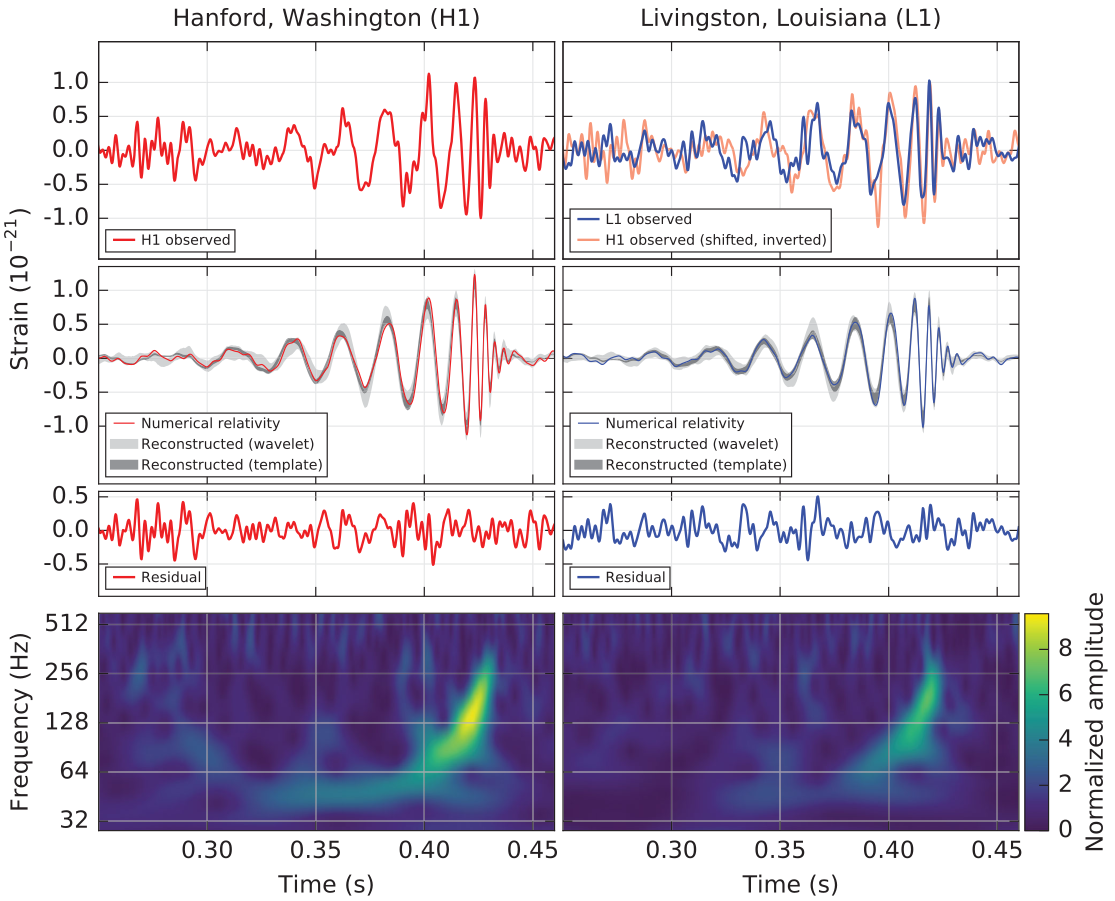
\includegraphics[width=\textwidth]{./images/GW150914.png}
	\caption{Signal detection of GW150914. \textit{Top:} amplitude time-series. \textit{Bottom:} frequency time-series. \cite{Abbott2016firstGW}}\label{fig:GW150914}
\end{figure}

\paragraph{GW150914-like binaries} It is possible to apply the above formulas to get an order-of-magnitude estimate of any binary detection. For instance, the Bayesian analysis of the signal of GW150914 reported in Fig.\ \ref{fig:GW150914} revealed two black holes of masses $M_1=35.6^{+4.7}_{-3.1} ~ \msun$ and $M_2=30.6^{+3.0}_{-4.4} ~ \msun$ at redshift $z=0.09^{+0.03}_{0.03}$ within 90\% confidence intervals. \cite{GWTC-1} Using Eq.\ \ref{eq:Massesredshift}, the masses revealed in the detector frame where about 10\% heavier, respectively $M_1 \sim 39 ~ \msun$ and $M_1 \sim 33 ~ \msun$. The corresponding chirp mass was $\mathcal{M} \sim 30 \msun$ and the total mass $M \sim 70 ~ \msun$, meaning that at the coalescence the binary had a radius of only $R_{\rm coalescence} \sim 200~\text{km}$ and produced a peak gravitational wave at $\nu_{\rm GW, peak} \sim 300 ~\text{Hz}$. The binary had a luminosity distance of $d_L=410~\text{Mpc}$ and the gravitational wave was detected with an amplitude of $h \sim 10^{-21}~ \text{Hz}^{-1/2}$.


\begin{figure}[h]
	\begin{minipage}{.47\textwidth}
		\centering
		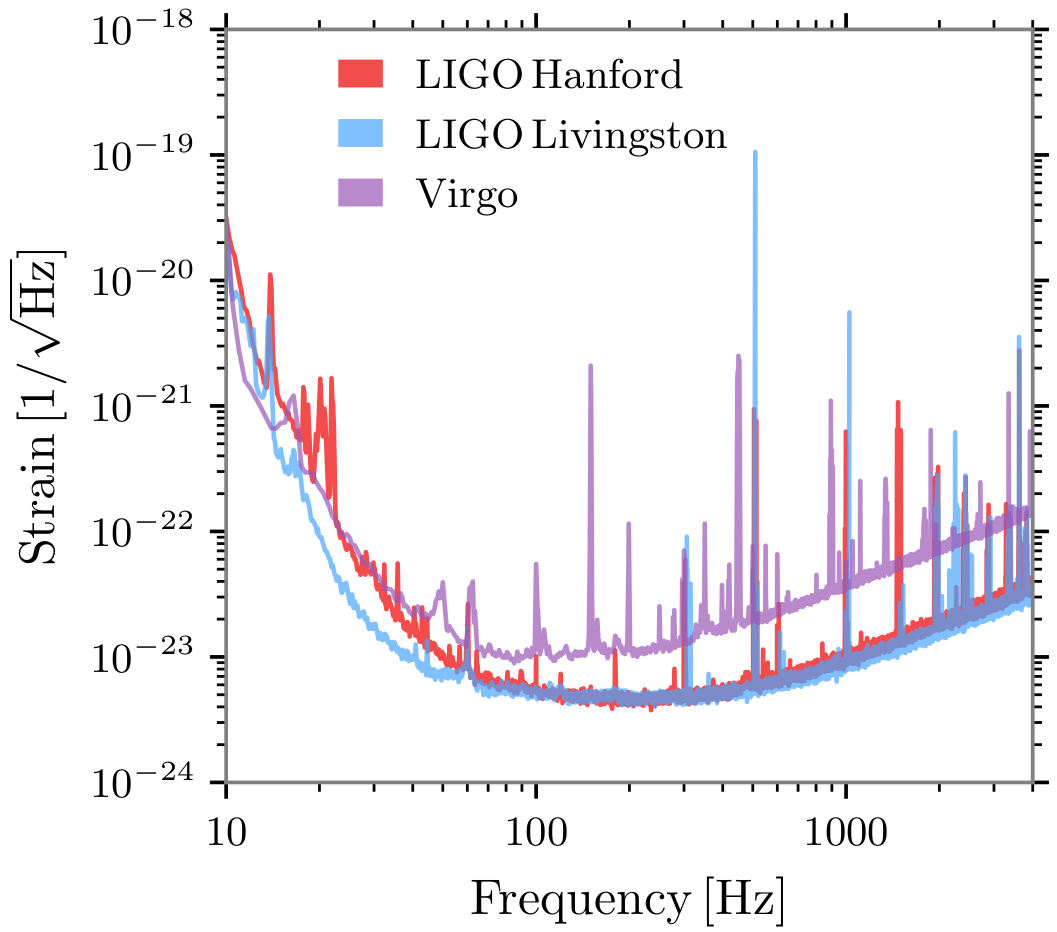
\includegraphics[width=\textwidth]{./images/sensitivity.png}
	\end{minipage}
	\hfill
	\begin{minipage}{.53\textwidth}
		\centering
		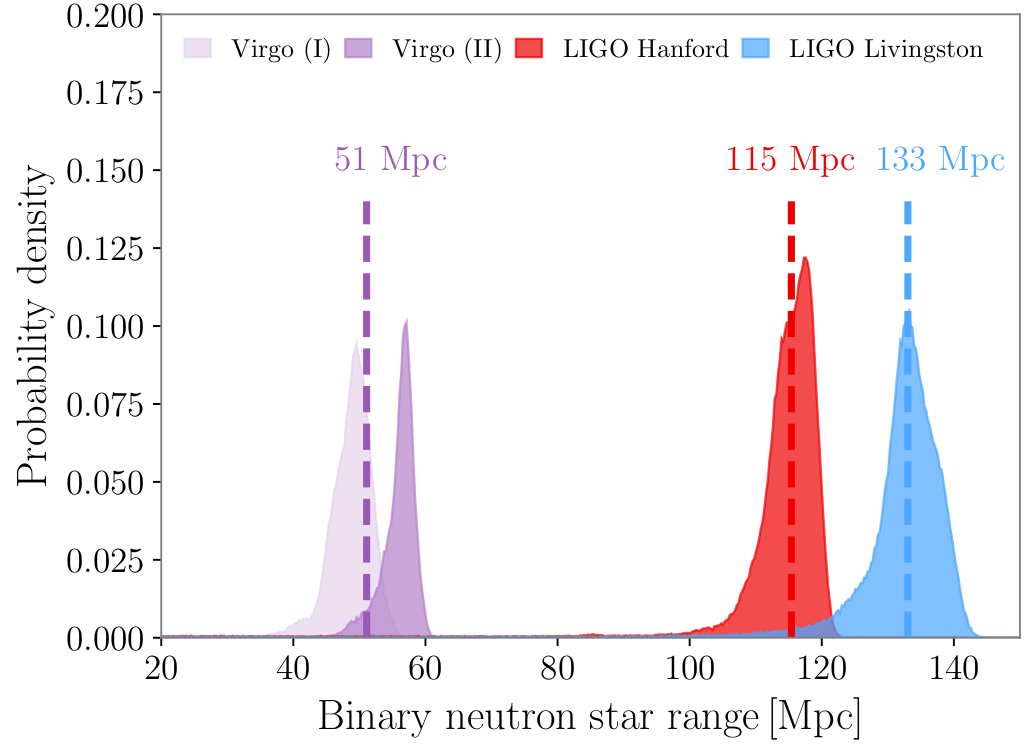
\includegraphics[width=1.02\textwidth]{./images/O3BNSrange.png}	
	\end{minipage}
	\caption{Sensitivity curves (\emph{left}) and binary neutron star observational probability density (\emph{right}) of the LIGO and Virgo interferometers during the third observing run O3. The lower sensitivity of Virgo for $\nu \gtrsim 150~\text{Hz}$ limits the observable volume, especially for the lighter sources like the binaries of neutron stars. \cite{GWTC-3}}\label{fig:O3sensitivity}
\end{figure}



\begin{figure}[h]
	\begin{minipage}{.49\textwidth}
		\centering
		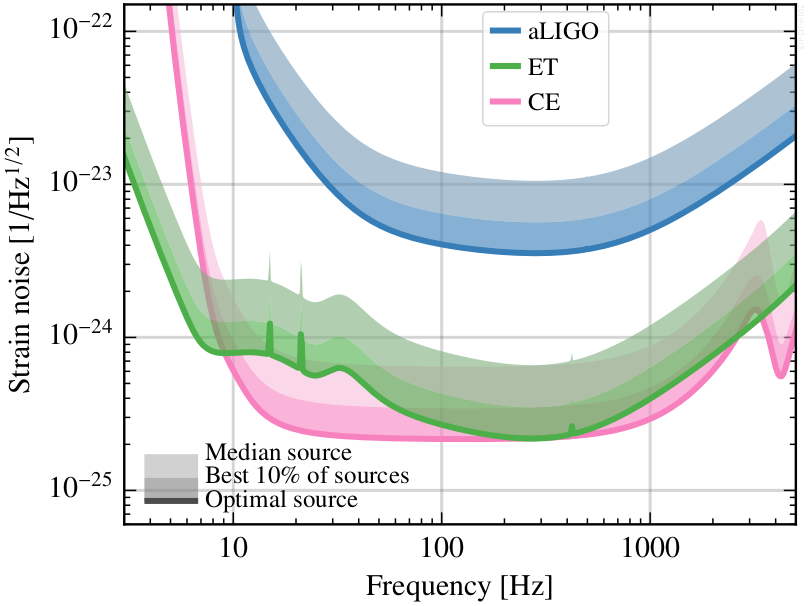
\includegraphics[width=\textwidth]{./images/ETsensitivity.png}
	\end{minipage}
	\hfill
	\begin{minipage}{.49\textwidth}
		\vspace{-2mm}
		\centering
		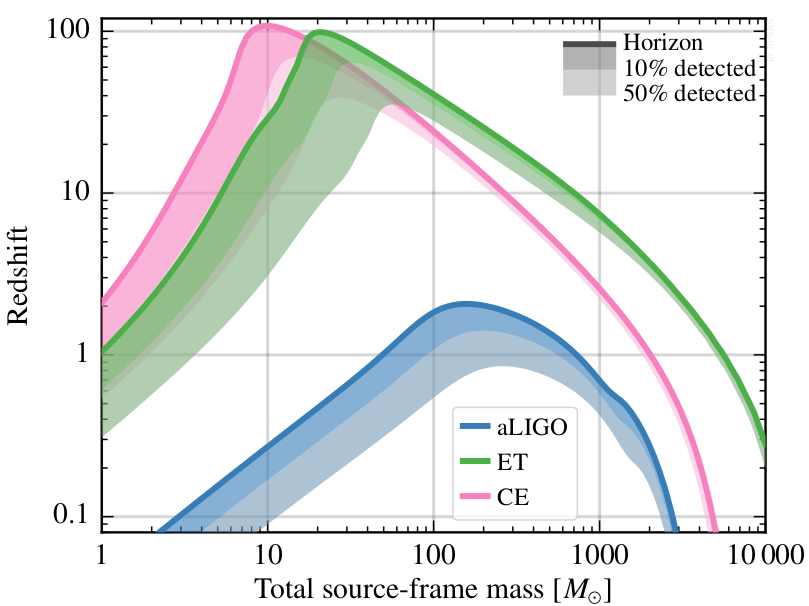
\includegraphics[width=1.02\textwidth]{./images/EThorizon.png}	
	\end{minipage}
	\caption{Example of the possible sensitivity curves (\emph{left}) and observable horizons (\emph{right}) of the planned third generation interferometers Einstein Telescope and Cosmic Explorer. Unlike the advanced LIGO interferometer, Einstein Telescope and Cosmic Explorer will detect for the first time black hole binaries well-beyond redshift $z \gtrsim 1$. \cite{EThorizonsensitivity}}\label{fig:ETsensitivity}
\end{figure}


\paragraph{Sensitivity, biases and future perspectives}
According to Eq.\ \ref{eq:h}, the further the sources and the lower the amplitude of the gravitational wave that reaches the detector.  To have a quantitative comparison it is useful to use as proxy-source a binary neutron star: the limits on its equation of state impose that a single neutron star has at maximum a mass of $\sim 3~\msun$, therefore the binary chirp mass is well-defined and doesn't exceed $\mathcal{M} \sim 2.6 ~\msun$. \cite{NSreview} Fig. \ref{fig:O3sensitivity} reports the sensitivity curves of the LIGO and Virgo interferometers and the end of the third observing run O3, highlighting how the worst sensitivity of Virgo at the high frequency (mainly caused by the photon shot noise) limits the maximum observable distance of the binary neutron star by a factor of 2 when compared to the performances of LIGO. \cite{GWTC-3} 

In terms of binary black holes, a source like GW150914 that peaks at $\nu \sim 300~\text{Hz}$ could be observed by the LIGO interferometers with sensitivity of $h \sim 10^{-23}~ \text{Hz}^{-1/2}$ up to a luminosity distance of $d_L \sim 1.6~\text{Gpc}$: the binary can now be observed in a volume of space $\sim 64$ times bigger. The observable volume is maximum for binaries that merge close to the best sensitivity range at $\sim 100-200~\text{Hz}$, that, according to Eq.\ \ref{eq:nupeak} are likely binaries composed of heavy black holes with total mass of $M \sim 100-200~\msun$: the gravitational wave detectors are biased towards the observation of heavy binary black holes.


Third generation gravitational wave detectors, like the planned Einstein Telescope and Cosmic Explorer, will be at least an order of magnitude more sensible than the refined versions of the LIGO and Virgo interferometers, allowing to probe the mergers of binary compact objects beyond redshift $z \gtrsim 1$. As shown in Fig.\ \ref{fig:ETsensitivity}, the maximum observable distance depends on the source mass and on the interferometers sensitivity, that ultimately depends on its design and is still under development (Fig.\ \ref{fig:ETsensitivity} is only one of the proposed designs, but is representative of the goals of the projects). \cite{EThorizonsensitivity} Again, Eq.\ \ref{eq:h} underlines how the detection improvement is mainly for the black hole binaries: their heavier mass produces stronger amplitude signals than the neutron star binaries, making them visible even at cosmic distances.



\subsection{Mass and spin observed distributions}\label{subsec:GWmassspin}%pluto

\paragraph{Merger rate densities and posterior distribution}
The parameter distributions of the observed gravitational wave sources are usually expressed either in terms of cumulative density functions or in terms of \emph{merger rate densities}. The merger rate densities represent the number of sources that merge in a comoving hypervolume and in a given parameter range. Given that the gravitational waves can be detected over different comoving hypervolumes depending on their frequency, chirp mass and detector sensitivity, the merger rate densities are the distribution functions that can better reproduce the intrinsic astrophysical ones.

Any distribution function is expressed in the form of a posterior probability and accounts for the many astrophysical and statistical limitations that affect the rough observed distributions. The corrections may enter as priors (like the intrinsic astrophysical population), likelihoods (like the signal-to-noise ratio that indicates the probability that each source is of astrophysical origin) or as normalization factors (like the correction for the sensible comoving hypervolume available for the detection, integrated for the observation time). In general, the observations are corrected for the limited sensitivity and detection efficiency but there is no extrapolation made to account also for the observational biases. \cite{GWTC-3}


\begin{figure}
	\begin{minipage}{.60\textwidth}
		\centering
		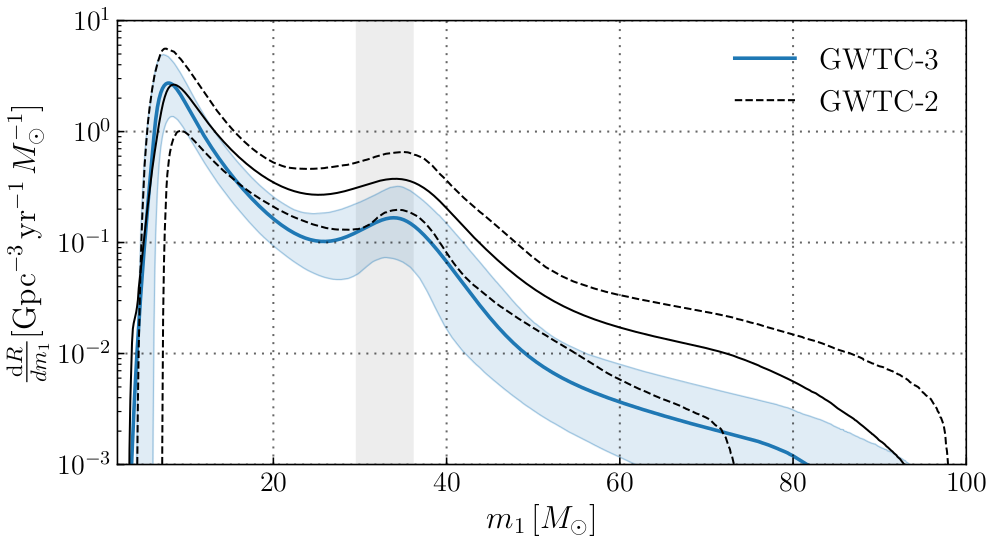
\includegraphics[width=\textwidth]{./images/MassMergerRate.png}
	\end{minipage}
	\hfill
	\begin{minipage}{.39\textwidth}
		\vspace{1mm}
		\centering
		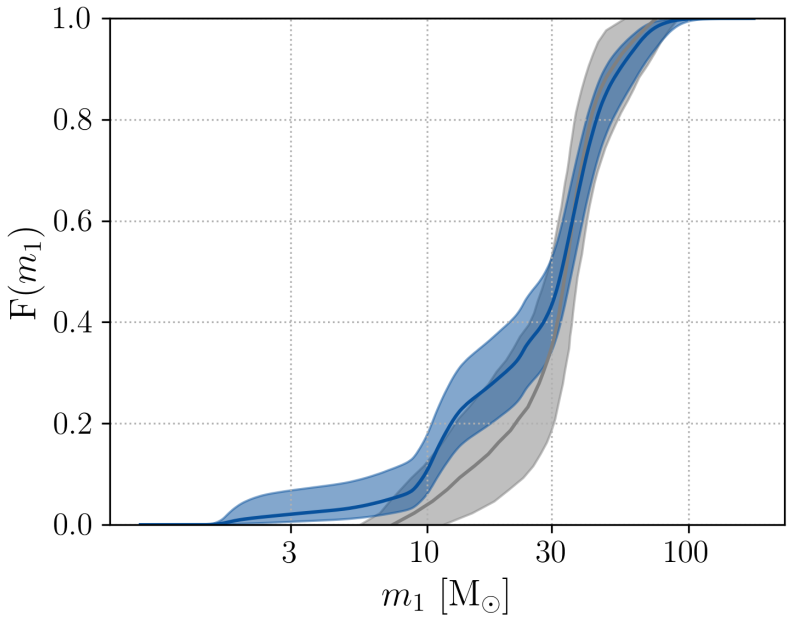
\includegraphics[width=\textwidth]{./images/MassCumulative.png}	
	\end{minipage}
	\caption{Differential merger rate (\emph{left}) and cumulative density function (\emph{right}) of the primary mass of the black hole binaries detected with the gravitational waves. In blue the posterior distributions obtained after the third observing run O3, in grey the ones obtained after O2. Thick solid lines denote the median values and are surrounded by the 90 \% credible intervals.The vertical grey band on the differential merger rate indicates the 90 \% credible interval for the mean of the Gaussian peak. \cite{GWTC-3_interpretation}}\label{fig:primarymassspectrum}
\end{figure}


\paragraph{Primary mass spectrum}
For each binary source, the primary mass is defined as the most massive one. Both the cumulative density function and the differential merger rate of the primary mass of the black hole binaries obtained at the end of the third observing run O3 are similar to the ones obtained at the end of the second observing run O2, as shown in Fig.\ \ref{fig:primarymassspectrum}. \cite{GWTC-3_interpretation}

The differential merger rate of the primary mass observed at the end of O3 is a power-law with slope $\alpha = 3.5_{-0.56}^{+0.6}$ with a Gaussian peak centered in $M_{\rm 1,\mu} = 34_{-4.0}^{+2.6}~ \msun$. GWTC-3 hosts more low-mass system than GWTC-2, causing a steeper decline in the power law at higher masses and reducing the mass of the 99th percentile, now at $\sim 44~\msun$ and not at $\sim 60~\msun$ as it was in GWTC-2. There are strong overdensities at $\sim 10~\msun$ and $\sim 35~\msun$ that may reflect properties of the astrophysical environment but that are still under investigation.

Even though the region $\gtrsim 70~\msun$ is still weakly explored, there is no strong evidence for or against a mass-gap, at least up to $\sim 75~\msun$. Still, a similar finding challenges the existence of the pair-instability mass-gap $\sim 60 - 120~\msun$ \cite{spera2017_pisnSNe}: either the single stellar evolution models need to be corrected \cite{MassGapStellarEvo_Costa2021} or the formation in dynamically active environments is required \cite{Rastello2021_dynamics}. On the other hand, there is still evidence of a lower-mass gap between $\sim 3~\msun$ and $\sim 5~\msun$, potentially due to the physics of core-collapse supernovae and in agreement with the dearth of compact objects observed in the galactic X-ray binaries \cite{massgapreal_ozel2010}.




\paragraph{Spin distribution}
At the end of the third observing run, the black hole population exhibits a preference for low-spinning black holes $\chi \lesssim 0.4$, with a peak distribution at $\chi \sim 0.2$ and a large tail at higher values. Separate analysis of the fastest ($\chi_A$) and slowest ($\chi_B$) spinning components of the binary revealed that the rapid-spinning components are still quite slow $\chi_A \sim 0.4$ while the slow-spinning ones are concentrated below $\chi_B \sim 0.2$, as expected. Posterior distributions for the spin magnitudes are shown in Fig.\ \ref{fig:spinmagnitude}.

The effective spin parameter $\chi_{eff}$ distribution is a Gaussian centered in $\chi_{eff, \mu} = 0.06_{-0.05}^{+0.04}$. The distribution peak is compatible with $\chi_{eff} = 0$, indicating spins misaligned with the orbital angular momentum. Detailed analysis required the existence of negative effective spins $\chi_{eff} < 0$, related to polar angles $\theta \geq 90^\circ $ and thus to black holes anti-aligned with the orbital angular momentum that likely formed in dynamically active environments. Moreover, data from GWTC-3 exhibit a mild anti-correlation between the effective spin parameter $\chi_{eff}$ and the mass ratio $q$, as shown in Fig.\ \ref{fig:spineffective}. If confirmed, the anti-correlation would challenge the usual evolutionary pathways for the binary black hole progenitors, indicating that field binaries formed with $q \sim 1$ don't have spins aligned with the orbital angular momentum ($\chi_{eff} \sim 1$),  because either the tides and mass transfer are not so efficient or there is some additional and yet un-considered effect, like a third-body perturbation \cite{misalignedbinary}. 



\begin{figure}
	\begin{minipage}{.49\textwidth}
		\centering
		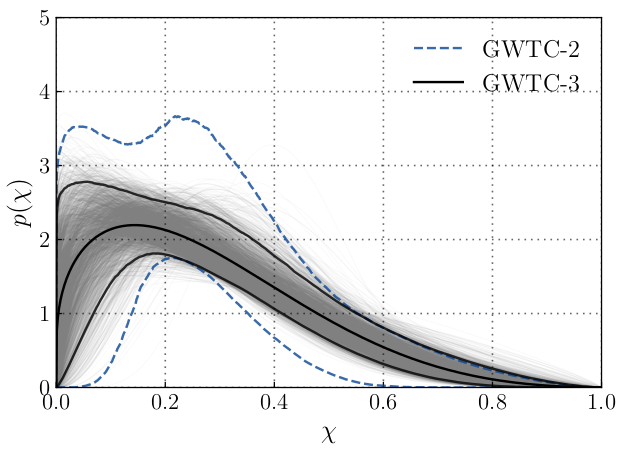
\includegraphics[width=\textwidth]{./images/spinmagnitude.png}
	\end{minipage}
	\hfill
	\begin{minipage}{.49\textwidth}
		\vspace{0.8mm}
		\centering
		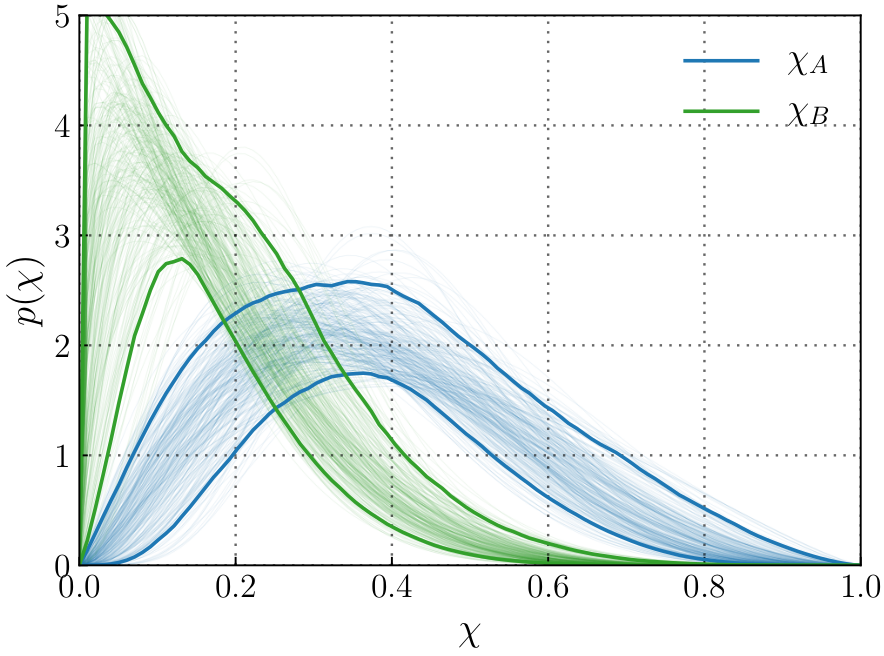
\includegraphics[width=0.975\textwidth]{./images/spinmagnitudehighlow.png}	
	\end{minipage}
	\caption{\emph{Left:} Spin magnitudes $\chi$ posterior distribution of all the merging black holes at the end of the third observing run O3 (in gray) compared to the 90 \% credible intervals for the sample limited at the end of O2 (in blue). \emph{Right:} Separate posterior distributions within 90 \% credible bounds of the fastest ($\chi_A$, in blue) and slowest ($\chi_B$, in green) black holes in the binaries. The new observations indicate a preference for slow-spinning black holes $\chi \lesssim 0.4$, with a fast-spinning component still rather slow $\chi_A \sim 0.4$ \cite{GWTC-3_interpretation}} \label{fig:spinmagnitude}
\end{figure}


\begin{figure}
	\begin{minipage}{.49\textwidth}
		\centering
		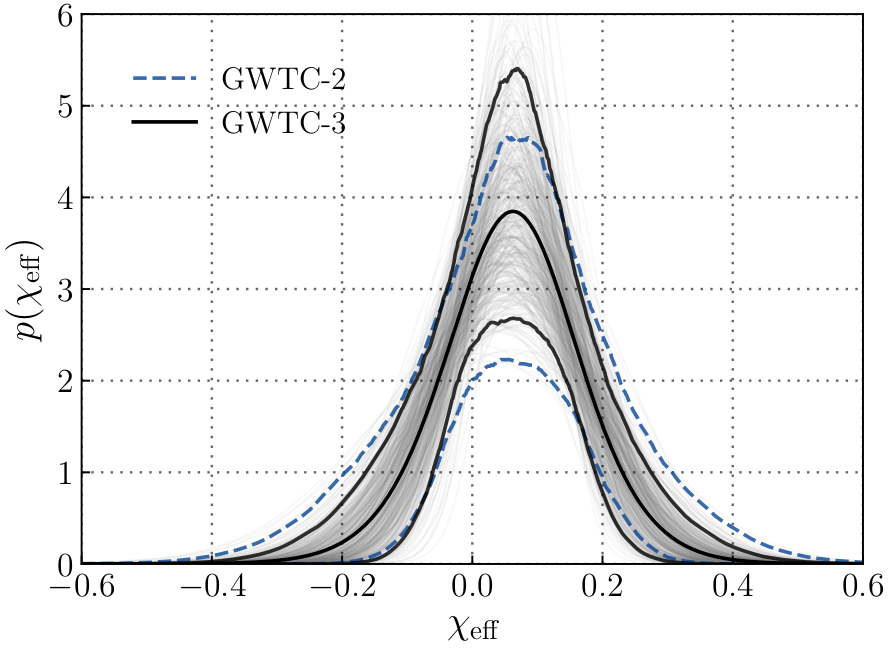
\includegraphics[width=\textwidth]{./images/spineff.png}
	\end{minipage}
	\hfill
	\begin{minipage}{.49\textwidth}
		\vspace{-1mm}
		\centering
		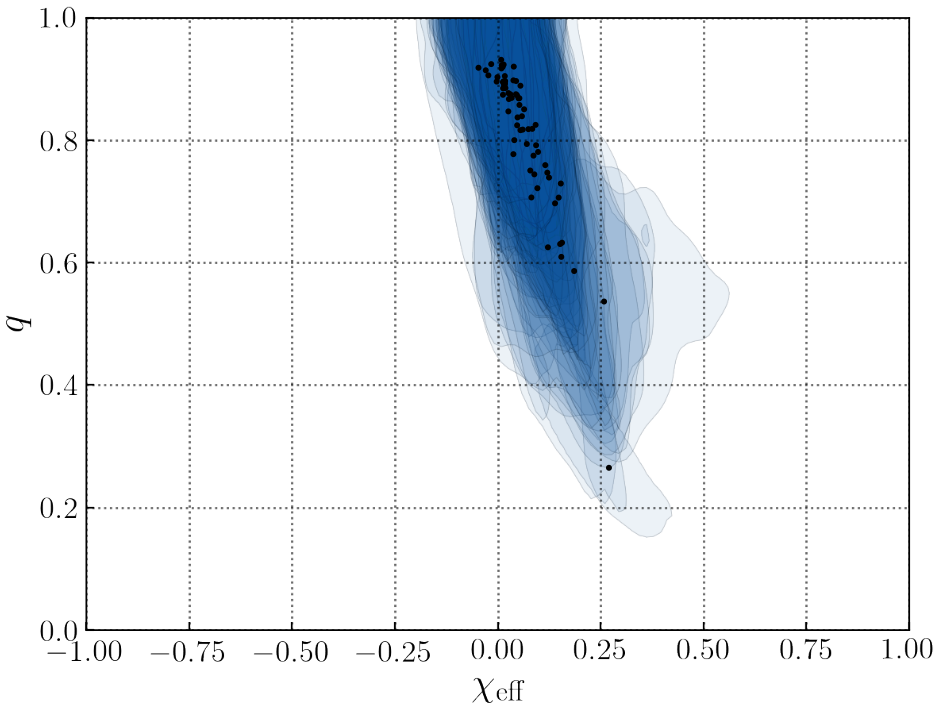
\includegraphics[width=0.96\textwidth]{./images/spinmassratio.png}	
	\end{minipage}
	\caption{\emph{Left:} Gaussian posteriors of the effective spin $\chi_{eff}$ of all the merging black holes at the end of the third observing run O3 (in gray) compared to the 90 \% credible intervals for the sample limited at the end of O2 (in blue). \emph{Right:} Effective spin $\chi_{eff}$ anti-correlating with the mass ratio $q$. Black points mark the median of the posterior distributions obtained using an informed prior where mean and standard deviation of the Gaussian posterior of $\chi_{eff}$ were allowed to evolve with $q$. Blue shaded areas indicate 90 \% credible intervals for each median point. \cite{GWTC-3_interpretation}} \label{fig:spineffective}
\end{figure}



The new detections included in the GWTC-3 catalogue strongly favour an isotropically oriented distribution of spins, as shown in the left panel of Fig.\ \ref{fig:spinorientation}. The scenario is consistent with the evolution in a dynamically active environment.

So far the analysis carried out assumed the same spin distribution at all masses, even though the low-mass binaries dominate the sample and seven high-mass binaries made up $\sim 70 \%$ of the moderate spins. A more refined analysis compared the spin magnitude aligned with the orbital angular momentum $|s_z|$ with the chirp mass of each binary. The result is shown in the right panel of Fig.\ \ref{fig:spinorientation}. All the binaries are consistent with spins misaligned with the orbital angular momentum ($|s_z| = 0$) even tough there are over-densities in the chirp mass distribution: if confirmed by further detections it would challenge the correlations predicted by the hierarchical formtion scenario. The large spread of the high-mass binaries $\mathcal{M} \gtrsim 30~\msun$ with respect to the low-mass ones is consistent with having a large number of detection at low masses and fewer at high masses: at the moment it is not possible to refute or confirm an aligned spin magnitude dependence with the chirp mass.






\begin{figure}
	\begin{minipage}{.49\textwidth}
		\centering
		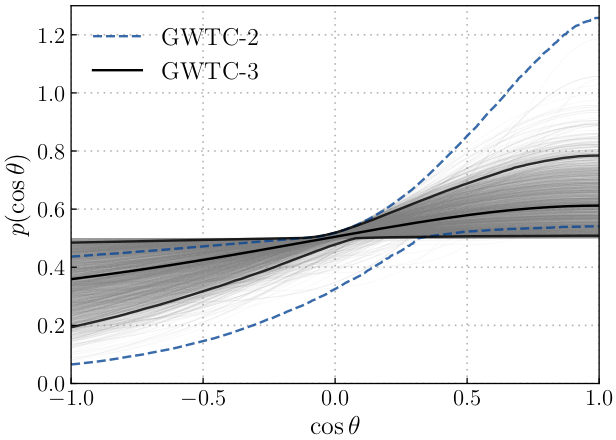
\includegraphics[width=\textwidth]{./images/spinorientation.png}
	\end{minipage}
	\hfill
	\begin{minipage}{.49\textwidth}
		%\vspace{-2mm}
		\centering
		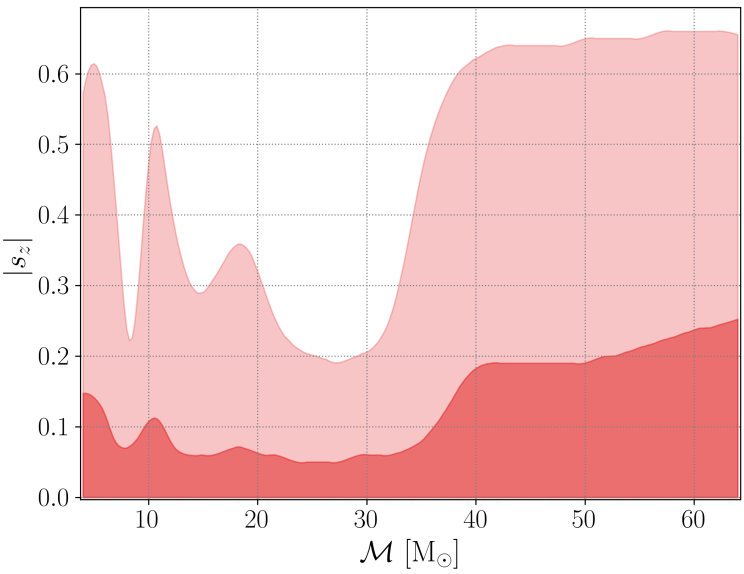
\includegraphics[width=0.95\textwidth]{./images/spinchirpmass.png}	
	\end{minipage}
	\caption{\emph{Left:} Posterior distribution of the polar angle $\theta$ of all the merging black holes at the end of the third observing run O3 (in gray) compared to the 90 \% credible intervals for the sample limited at the end of O2 (in blue). \emph{Right:} Spin magnitude aligned with the orbital angular momentum $|s_z|$ as a function of the binary chirp mass. Light(dark) shaded areas indicate 90 \% (50 \%) credible intervals. \cite{GWTC-3_interpretation}}\label{fig:spinorientation}
\end{figure}






\section{X-ray binaries}
\subsection{X-ray binaries hosting a black hole}\label{subsec:XraybinariesSED}
\paragraph{The best way to observe a black hole}
X-ray binaries that host a black hole are currently the best observational candidates as binary black hole progenitors: not only such systems are already in a binary configuration but the accretion onto the compact object powers an X-ray emission that allows us to observe them \cite{Xbinaries_massmeasure}. Observability is precisely the key property of the X-ray binaries: even though $\sim 70 \%$ of the massive stars are born in binary systems \cite{Sana2012}, many black holes are quiescent and can be observed only with accurate radial velocity measurements \cite{BHnoninteracting_Giesers2018}. Isolated black holes, that could dynamically exchange with a binary, are even more difficult to observe and currently the best detection technique is microlensig \cite{BHmicrolensing}.

\paragraph{LMXBs and HMXBs}
The mass of the non-degenerate donor star and the type of the accretion determine two sub-classes of X-ray binaries hosting a black hole: Low-Mass X-ray Binaries (LMXBs) and High-Mass X-ray Binaries (HMXBs). LMXBs typically have low-mass stars $\lesssim 2-3~\msun$ that fill their Roche Lobe. HMXBs donors, on the contrary, are more massive stars $\gtrsim 5~\msun$ that don't fill their Roche Lobe but become wind-fed systems. Up-to-date, about $\sim 30$ X-ray binaries are known to host a black hole \cite{HMXBH_spins2021}.

\paragraph{Spectral energy distribution in the X-rays}
The X-ray spectral energy distribution of an X-ray binary is dominated by the emission of the accretion disk surrounding the compact object. A classic Shakura-Sunyaev accretion disk emits most of its photons in the UV/soft X-ray regime $\sim 10^{2}-10^{4}$ keV with an X-ray luminosity $L_X \gtrsim 10^{37}~\text{erg s}^{-1}$, has an effective radiation temperature of $\sim 10^{7}-10^{8}~K$ and produces a thermal multi-color blackbody continuum \cite{S&S1973_accretiondisk}. Usually the accretion disks are surrounded with a corona of hot thermal electrons: photons in the low energy tail of the disk thermal emission (soft optical/UV) that encounter the corona suffer multiple inverse Compton scatterings (i.\ e.\ suffer a thermal Comptonization) and are re-emitted in the form of a hard X-ray power-law spectrum. Part of the X-ray power-law radiation is directly emitted towards the observer at infinity but another part is re-emitted back to the accretion disk, reprocessed by it and eventually reflected at the infinity. 
 
The X-ray photons reprocessed by the corona are more energetic than the ones originally produced in the accretion disk and see the disk as a slab of cold gas, interacting with it mainly through Compton scattering and photoelectric absorption followed by fluorescent line emissions. On the one hand, the energy dependence of the photoelectric absorption favors the absorption of the soft X-rays, causing a down-scaling in the corresponding region of the reflected continuum. One other hand, the hard X-rays are Compton-scattered back, thus reflected towards the observer at the infinity, except for the ones more energetic than $\sim 20-30$ keV, that suffer the Compton recoil. Overall, the X-ray continuum due to the reflection is characterized by a hump at $\sim 20$ keV and by the fluorescent lines emitted by the ionized heavy elements, mainly iron. The 6.4 keV line of the Fe K$\alpha$ line is the strongest fluorescent line and is caused by the absorption of an incident photon with energy larger than 7.1 keV, as shown in the right panel of Fig. \ref{fig:accretiondisk}.

The X-ray continuum seen by an observer at infinity can be divided into the soft and hard X-ray regions, respectively below or above 10 keV. The soft X-ray spectrum is dominated by the thermal continuum of the disk and exhibits a multi-color black body shape peaked at $\sim 2$ keV. The hard X-ray spectrum is determined by the radiation reprocessed by the hot corona: the hard power-law of the photons directly emitted from the corona is modulated by the hump at $\sim 20$ keV and the fluorescence emission lines caused by the additional reflection on the accretion disk, as shown in the left panel of Fig. \ref{fig:accretiondisk}. \cite{FeKalphaline_Fabian2000}


\begin{figure}
	\begin{minipage}{.58\textwidth}
		\centering
		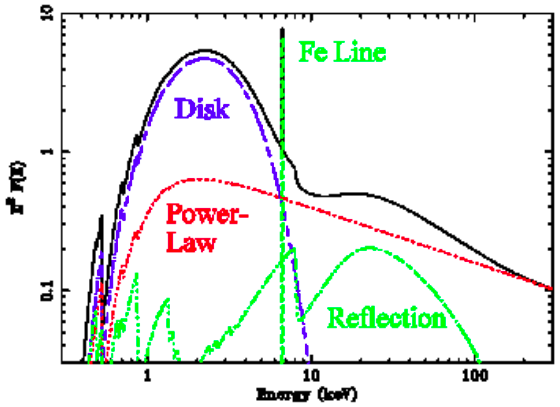
\includegraphics[width=\textwidth]{./images/accretiondiskSED.png}
	\end{minipage}
	\hfill
	\begin{minipage}{.42\textwidth}
		%\vspace{-2mm}
		\centering
		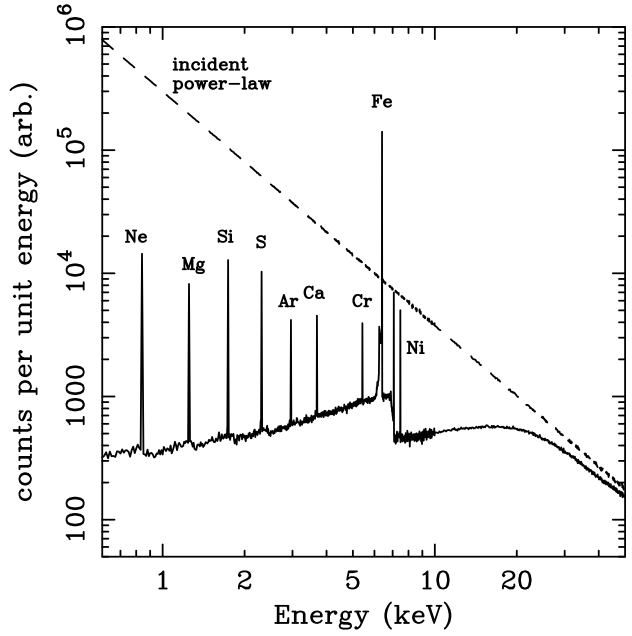
\includegraphics[width=\textwidth]{./images/accretiondiskFeKalphaline.png}	
	\end{minipage}
	\caption{\emph{Left:} Sketch of the dominant components in the spectral energy distribution of a X-ray binary. In the soft X-ray the emision is dominated by the thermal continuum of the disk, visible as a multi-color blackbody peaked at $\sim 2$ keV. In the hard X-ray, the radiation reprocessed by the corona is either directly emitted towards the observer as power-law or is reflected by the disk, causing a hump at $\sim 20$ keV and the strong fluorescent Fe K$\alpha$ line at $6.4$ keV. Credit: J. Miller \emph{Right:} Montecarlo simulation of the X-ray spectrum reflected by a cold slab of gas. An incident power-law radiation (dashed line) is damped in the soft X-rays, exhibiting strong fluorescent lines an a hump before the cut-off due to the Compton recoil. \cite{FeKalphaline_Fabian2000}}\label{fig:accretiondisk}
\end{figure}

\subsection{Measuring the properties of the X-ray binaries}\label{subsec:Xraymeasure}
\paragraph{Masses, period and inclination}
Inspection of the radial velocity and X-ray light curves provides essential informations to characterize the orbital properties of the X-ray binaries. On the one hand, the period can be directly obtained from the periodicity of the light and velocity curves and often is the most-accurate orbital parameter. On the other hand, the mass estimates of the black holes are less precise and rely on the determination of many other uncertain quantities, like the companion mass, binary mass ratio, inclination and distance.

The dynamical method is the most robust and common procedure to determine the mass of an object in a binary system. Its application is limited to the systems that satisfy three conditions: the companion star is visible in the optical/near-infrared band, single spectral lines can be identified in its optical/near-infrared spectrum (resolving power $\lambda/\Delta \lambda \gtrsim 1500$), at least one photospheric absorption line can be used as proxy for the orbital motion. Therefore, the dynamical method cannot be applied to distant X-ray binaries (not enough resolving power), to systems with a companion not visible in the optical/near-infrared band and, most importantly, to systems subject to outburst or strong stellar winds. These limitations prevent the application of the dynamical mass determination to many high mass X-ray binares. For instance, as explained in Sec.\ \ref{sec:WRBHobserved}, the strong winds of the Wolf-Rayet stars coupled with the X-ray variability of the compact object caused the revision of many dynamical mass measurement in the Wolf -Rayet - black hole binaries \cite{ICX10X-1_Laycock2015_revisited}.

Alternative techniques for the mass measurement are available but still require a good calibration, as for the case of the scaling relations with the X-ray spectral and timing properties \cite{Xbinaries_massfromXtiming}.\\

In the dynamical method, the spectral lines that trace the orbital motion are used to build the velocity curves and extract the orbital period $P_{orb}$ and the radial velocity semi-amplitude $K_c$ of the companion star. Kepler's third law corrects the measures for the inclination angle $i$ and the mass ratio $q=M_c/M_{\rm BH}$ and couples them into the \emph{mass function} $f(M)$: a non-linear expression relating the masses of the companion star $M_c$ and of the compact object $M_{\rm BH}$

\begin{equation}\label{eq:massfunction}
	f(M) = \frac{K_c^3 P_{\rm orb}}{2 \pi G} = \frac{M_{\rm BH}^3 \sin^3 i}{(M_{\rm BH} + M_c)^2} = \frac{M_{\rm BH}^3 \sin^3 i}{(1+q)^2}
\end{equation}

The above formula is for a circular binary: a reasonable assumption for a system that likely already had the time to circularize, given that its X-ray visibility is the result of a mass transfer process. Eventually, the mass of the black hole in the binary can be determined with further assumptions and measurements on the mass ratio $q$ (or, alternatively, on the companion mass $M_c$) and on the inclination of the system $i$.\\

The mass ratio can be determined assuming a spherically symmetric star that fills its Roche lobe in a tidally locked system. Under these conditions, the rotational broadening ($V \sin i$) of the absorption lines in the stellar photosphere can be related to the mass ratio $q$ of the system \cite{Xbinaries_qmeasure}

\begin{equation}\label{eq:qmeasure}
	\frac{V \sin i}{K_c} \sim 0.462~q^{1/3} (1+q)^{2/3} 
\end{equation}

The measurement of $q$ is not always feasible and usually leads to under-estimate its value. The main uncertainty arises from the assumption of sphericity in a Roche Lobe filling system that, on the contrary, has tidal distortions. Moreover, the rotational broadening is usually of $\sim 30-120~\text{km s}^{-1}$ and requires a very large resolving power $\lambda/\Delta \lambda \gtrsim 5000$ to be measured, limiting the determination of $q$ only to the nearest binaries. 

For many systems, including the HMXBs that are not filling their Roche Lobe, the mass function is not calculated with the mass ratio but with the companion mass. Fits on the stellar spectrum or mass-luminosity relations can provide the mass of the companion star. Nevertheless, also this result is a big source of uncertainty, especially for the HMXBs: the strong winds and mass lost deeply modify the photosphere of the star, therefore the synthetic spectra based on single stellar evolution models or the empirical mass-luminosity relations might be incorrect.\\


The inclination angle $i$ is usually obtained fitting the optical/near-infrared light curves with synthetic ellipsoidal model. Assuming that the companion star is filling its Roche Lobe, tidal deformations of the star surface are expected to modulate the light curve profile and the amplitude of the modulation can be linked to the inclination angle. The light curve modulation can be affected by many sources of error (outburst, winds, etc.) and requires a very complex modeling, resulting in inaccurate determinations of the inclination angle.  Unless the system it is an eclipsing binary, it inclination angle is poorly constrained and, given the cubic dependence in the mass function of Eq.\ \ref{eq:massfunction}, provides the biggest source of uncertainty in the black holes mass determination. \cite{Xbinaries_massmeasure}\\


HMXBs usually do not fill their Roche lobe and power the accretion through strong stellar winds: not only the method just described would provide very uncertain determinations for the inclination angle and companion mass but it would result in a very imprecise measure of the black hole mass. Therefore, the mass of the compact object in HMXBs is usually the result of a multi-parametric fit to the radial velocity curve and to the optical/near-infrared and X-ray light curves. The distance of the source is one of the parameters included in the multi-parametric model and the fit result is very sensible to it. For instance, recent radio astrometric distace measurements re-defined Cyg X-1 as a system hosting an O-type star of $\sim 40~\msun$ with a black hole of $\sim 21~\msun$, making it the most massive black holes detected so far in a X-ray binary \cite{cygnusx1}.




\paragraph{Spin}
Two techniques are generally used to measure the spin of the black holes and require a fit to the X-ray spectrum of the accretion disk, either on the continuum or on the Fe K$\alpha$ lines (see Sec.\ \ref{subsec:XraybinariesSED} for a more detailed description of the X-ray spectral energy distribution). Both methods assume a geometrically thin disk, radiatively efficient and with emission that terminates at the innermost stable circular orbit (ISCO): the faster the rotation of a Kerr black hole, the closer the ISCO. \cite{Xbinaries_spinBHmeasure}\\

The Fe K$\alpha$ line at 6.4 keV is a very strong fluorescent line produced by the X-ray radiation reflected from the accretion disk. In principle the line is very narrow but it is broadened by the Doppler effect, due to the disk rotation, and by the gravitational redshift, due to the vicinity to the black hole. Fast spinning Kerr black holes have a ISCO that is both closer to the black hole and more rapidly rotating, enhancing respectively the gravitational redshift and the Doppler shift. As shown in the left panel of Fig.\ \ref{fig:spinmeasure}, the spin of the black hole can be reconstructed by carefully fitting the broadening of the Fe K$\alpha$ line in the reflected X-ray spectrum.

The fit to the reflection spectrum has the great advantage of being a \textit{relative} measurement. Moreover, the spin determination can be carried out without knowing a priori the black hole mass, its distance and accretion rate, allowing the spins to be inferred in many system with poorly constrained black hole masses \cite{HMXBH_spins2021}. On the contrary, the emissivity and ionization of the disk need to be already modeled to provide a good fit. Reflection spectra are also very sensitive to the inner disk inclination, although this information can be extracted by the same fit used for the Fe K$\alpha$ line.\\

Spin determination through the fit of the hard continuum relies again on having a ISCO of the disk closer to the black hole for high spin values. The thermal emission of the disk can be modeled as a multi-color blackbody, where each anulus emits as a thermal blackbody with radiation temperature $T \propto r^{-3/4}$ hotter for anuli closer to the black hole. Fast rotating black holes have accretion disks with ISCO very close to the black horizon that, being hotter, shift the peak of the multi-color emission towards higher energies: fitting the absolute shift in the flux emitted in the hard X-rays results in the spin determination, as shown in the right panel of Fig.\ \ref{fig:spinmeasure}.

The method has many drawbacks, the main one being its necessity to fit the \textit{absolute} flux shift in a region where the emitted flux is strongly influenced also by the hard power-law emitted by the corona (see the left panel of Fig.\ \ref{fig:accretiondisk} for a comparison): the choice of the hard component strongly impacts the spin value. Further sources of uncertainty come from the a priori knowledge of the inner disk inclination, atmospheric scattering corrections and, most importantly, mass and distance of the black hole, required to have an accurate model for the absolute flux emitted by the disk. \cite{Xbinaries_spinBHmeasure}




\begin{figure}
	\begin{minipage}{.48\textwidth}
		\centering
		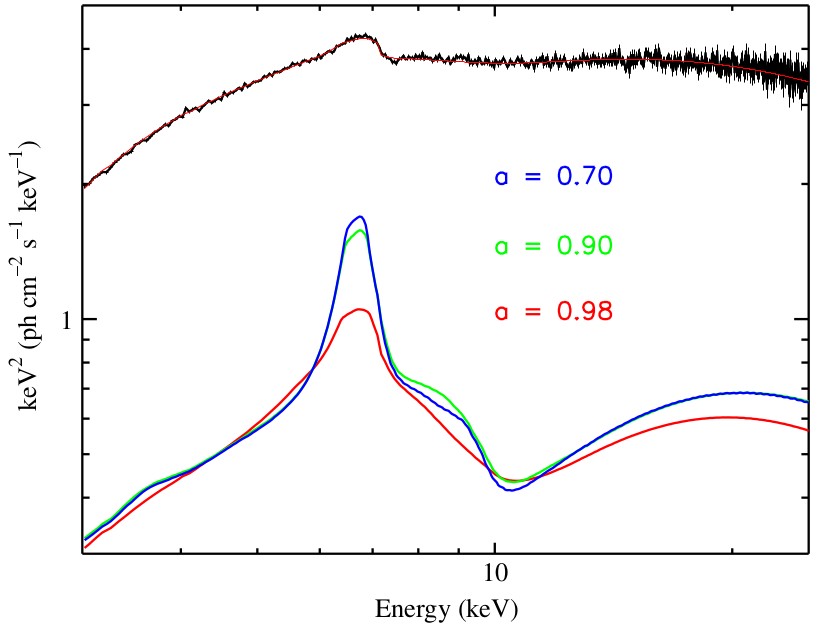
\includegraphics[width=\textwidth]{./images/spinreflection.png}
	\end{minipage}
	\hfill
	\begin{minipage}{.49\textwidth}
		%\vspace{-2mm}
		\centering
		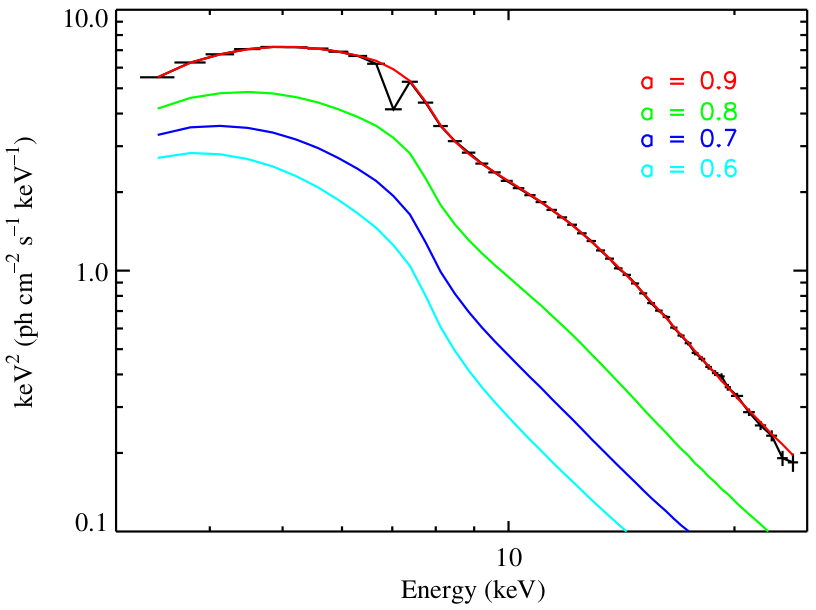
\includegraphics[width=\textwidth]{./images/spincontinuum.png}	
	\end{minipage}
	\caption{Example of the black hole spin measurement from fits to the Fe K$\alpha$ line (\emph{left}) or to the X-ray hard continuum (\emph{right}) of the candidate X-ray binary GRS 1915+ 105. The Fe K$\alpha$ fluorescent line causes the absorption at $\sim 7$ keV in the right panel and results in a strong, broadened emission centered at 6.4 keV in the left panel. The spectrum on the left is obtained with \textit{NuStar} while the one on the right with \textit{RXTE}. \cite{GSR1915_lowhardXstate}}\label{fig:spinmeasure}
\end{figure}


\section{Tensions in the underlying populations}%pluto
Up-to-date, one of the most detailed analysis of the mass and spin distribution of the underlying binary black hole populations compared the data of 44 binary black holes of the GWTC-2 catalogue with the only X-ray binaries with a reliable mass or spin measurement: 29 LMXBs and 3 HMXBs (see Sec.\ \ref{subsec:Xraymeasure} for a discussion on the main uncertainties in the X-ray parameter estimation) \cite{HMXBH_spins2021}. The study included as HMXBs the X-ray binaries with O-type donor star LMC X-1, M33 X-7 and Cyg X-1, excluding the Wolf-Rayet - black hole binaries like NGC 300 X-1 or IC 10 X-1 because they have a less reliable mass measurements \cite{ICX10X-1_Laycock2015_revisited} (see the discussion in Sec.\ \ref{sec:WRBHobserved}). Even though the binary black hole sample is limited to GWTC-2 \cite{GWTC-2}, it is reasonable to expect that the same conclusions can be obtained using the GWTC-3 data, as discussed in Sec.\ \ref{subsec:GWmassspin}. On the contrary, the limited sample of X-ray binaries with reliable mass and spin measurements causes the largest uncertainties.


\begin{figure}[h]
	\begin{minipage}{.49\textwidth}
		\centering
		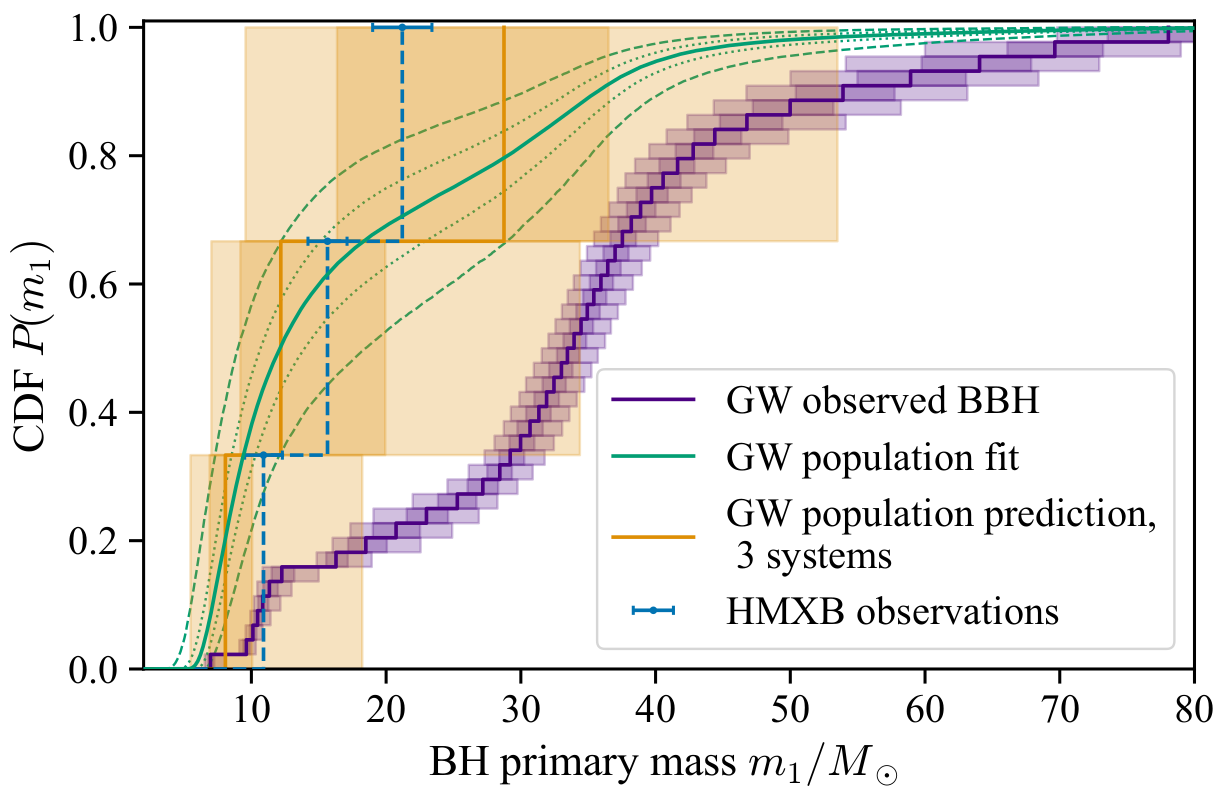
\includegraphics[width=\textwidth]{./images/tensionHMXBHmass.png}
	\end{minipage}
	\hfill
	\begin{minipage}{.49\textwidth}
		\vspace{.5mm}
		\centering
		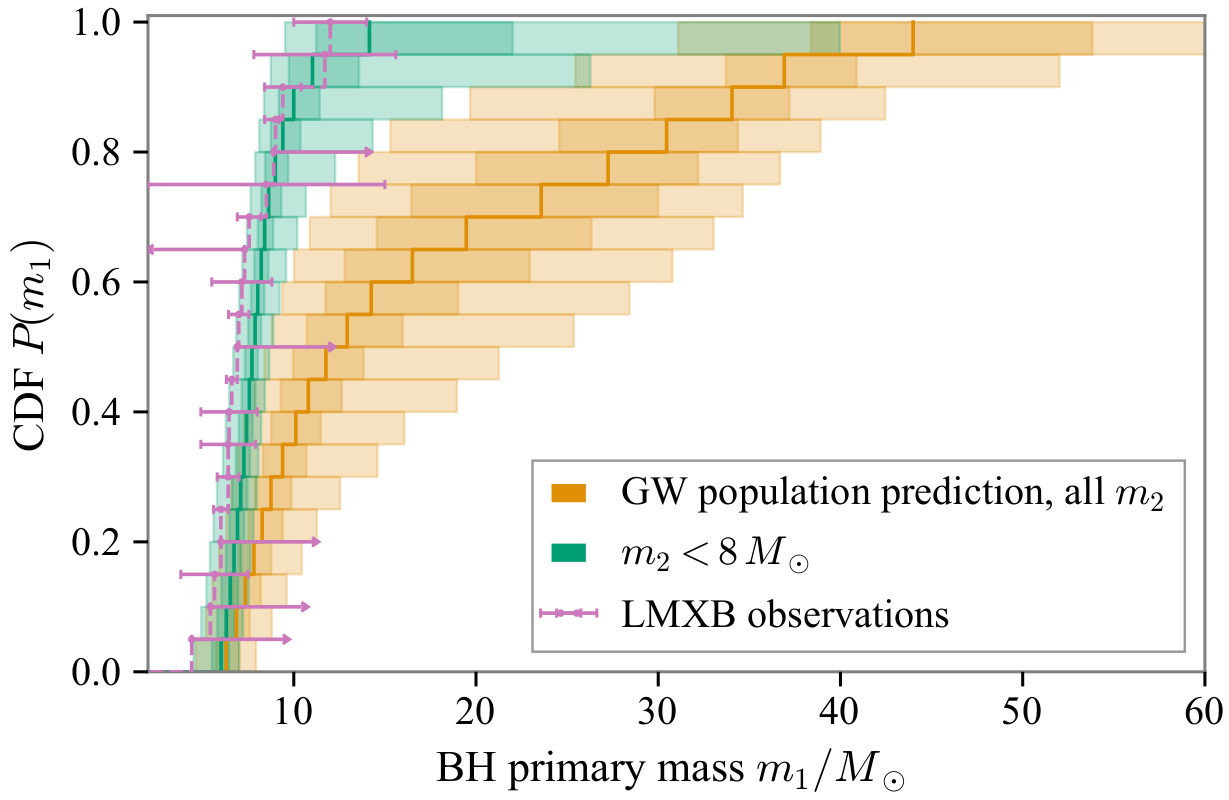
\includegraphics[width=\textwidth]{./images/tensionLMXBHmass.png}	
	\end{minipage}
	\caption{Observed cumulative distribution function (CDF) of the observed HMXBs (blue, \emph{left} panel) and LMXBs (pink, \emph{right} panel) compared with the CDFs (orange bands) expected if the X-ray binaries share the same primary black hole mass distribution of the primaries in the black hole binaries detected with the gravitational waves, once it is corrected for the selection effects (green line). In the left panel, the purple bands show the original observed CDF for black hole binaries not yet corrected for observational effects. In the right panel, the green bands show the CDF extracted from the sub-sample of the black hole binaries with secondary mass $< 8~\msun$. Dark (light) shaded areas delimit 50 \% (90 \%) credible intervals. \cite{HMXBH_spins2021}}\label{fig:tensionmass}
\end{figure}

\subsection{Similarities in the mass distribution}
The mass distribution of the primary (more massive) black hole of the black hole binaries detected with the gravitational waves seems compatible with the mass distribution of the black holes detected in the LMXBs and HMXBs, once the corrections for gravitational wave selection effects and similar mass pairing are taken into account. If confirmed, the relation would indicate that X-ray binaries hosting a black hole could be the progenitors of the black hole binaries detected with the gravitational waves. However, the small sample of X-ray binaries with reliable mass measurements ($\sim 30$) is affected by a large Possion uncertainty, possibly hiding inconsistencies in the underlying populations. Moreover, observational selection effects on the X-ray binaries are not accounted for and may further change the degree of consistency. \\

The left and right panel in Fig.\ \ref{fig:tensionmass} show the agreement between the cumulative distribution functions (CDF) of the primary black hole population underlying in the gravitational wave observations and the CDFs for the black hole population underlying in the HMXBs and LMXBs, respectively. The observed CDF of the 44 black hole primaries considered in the GWTC-2 (purple bands in the left panel of Fig.\ \ref{fig:tensionmass}) is corrected for the observational selection effects that favor the detection of gravitational waves produced by heavy black holes (see Sec.\ \ref{subsec:GWtheorymethod}). The corrected posterior CDF (green line in the left panel of Fig.\ \ref{fig:tensionmass}) is indeed shifted towards lower masses and describes the \textit{intrinsic} primary mass distribution of the black holes detected with the gravitational waves. 

The observed CDFs of HMXBs and LMXBs (respectively the blue/pink dashed lines in the left/right panel of Fig.\ \ref{fig:tensionmass}) cannot be directly compared with the intrinsic CDF of the primary black hole masses. The considered sample of HMXBs and LMXBs contains, respectively, only 3 and 29 black holes: their CDFs are dominated by the Poisson uncertainty if they are extracted from the same intrinsic population of the black hole binaries. To account for Poisson noise, many sets of 3 or 29 black holes are randomly extracted from the intrinsic black hole binary distribution (the green line already found). Each set is then used to build a CDF. Subsequently, all the extracted CDFs of 3(29) black holes are put together to reconstruct a CDF representative of the black holes in HMXBs(LMXBs) than will become primary black holes in the black hole binary systems detected with the gravitational waves (orange bands in both the panels of \ref{fig:tensionmass}). The extracted CDFs have very large credible intervals, as expected from the huge Poissonian noise acting on the limited sample of the X-ray binaries. \\

On the one hand, the left panel of Fig.\ \ref{fig:tensionmass} shows that the observed mass distribution of the black holes in HMXBs (blue) is compatible within 50 \% credible intervals with the distribution expected if the black holes of the HMXBs become the primaries of the black holes binaries detected with the gravitational waves (orange). On the other hand, the right panel of Fig.\ \ref{fig:tensionmass} shows that LMXBs seem to have an observed black hole mass distribution (pink) too much shifted in the lower masses with respect to the one expected from being a progenitor of the black hole binaries (orange). However, the discrepancy is removed if the expected CDF is not extracted from all the 44 black hole binaries but only from the binaries with light secondary black holes $M_2 < 8~\msun$ (green bands). The selection of the sub-sample of binaries is justified because isolated binaries seems to favor the production of similar masses remnants and the LMXBs already host a low-mass secondary $\lesssim 2-3~\msun$. Even though secondary stars so light will unlikely produce black holes up to $8~\msun$, the agreement in the CDFs could suggest that possible differences in the LMXBs and binary black hole masses may be caused by the mass of the secondary star and not by the mass of the primary black hole. \cite{HMXBH_spins2021}



\begin{figure}
	\begin{minipage}{.49\textwidth}
		\centering
		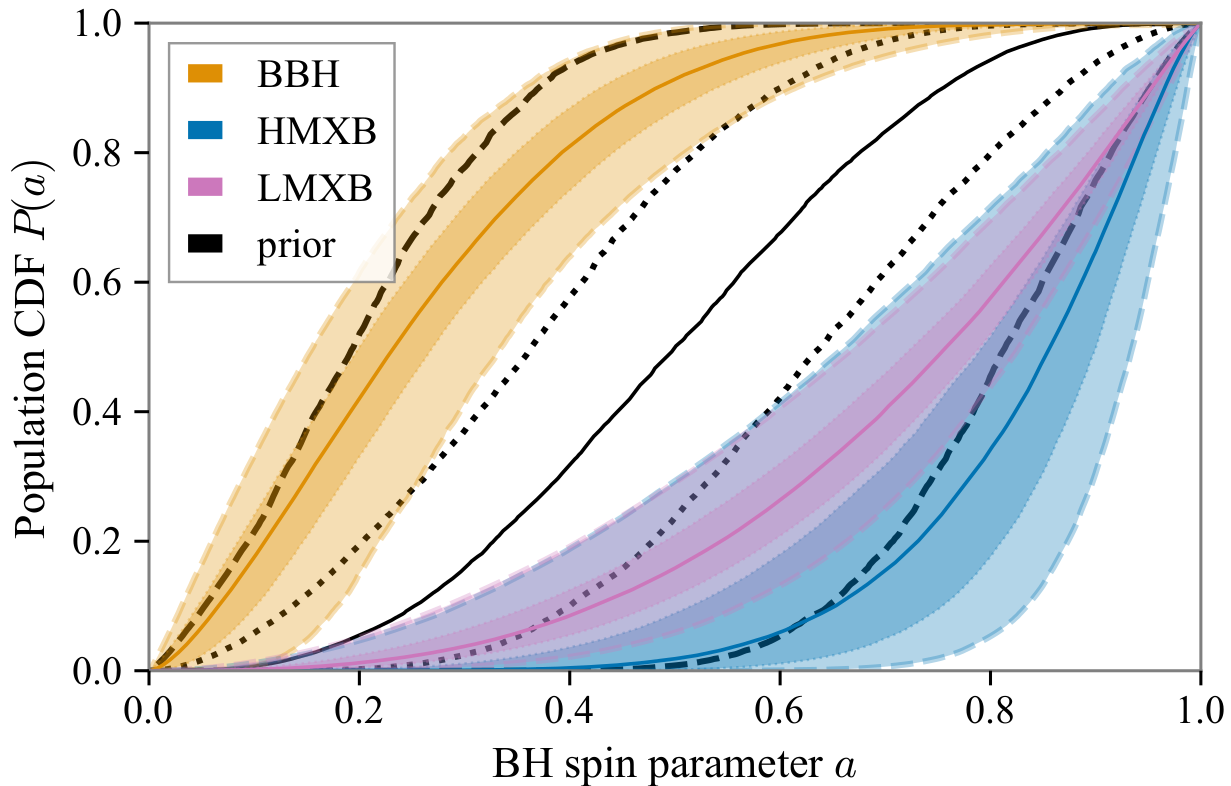
\includegraphics[width=\textwidth]{./images/tensionspin.png}
	\end{minipage}
	\hfill
	\begin{minipage}{.49\textwidth}
		\vspace{.5mm}
		\centering
		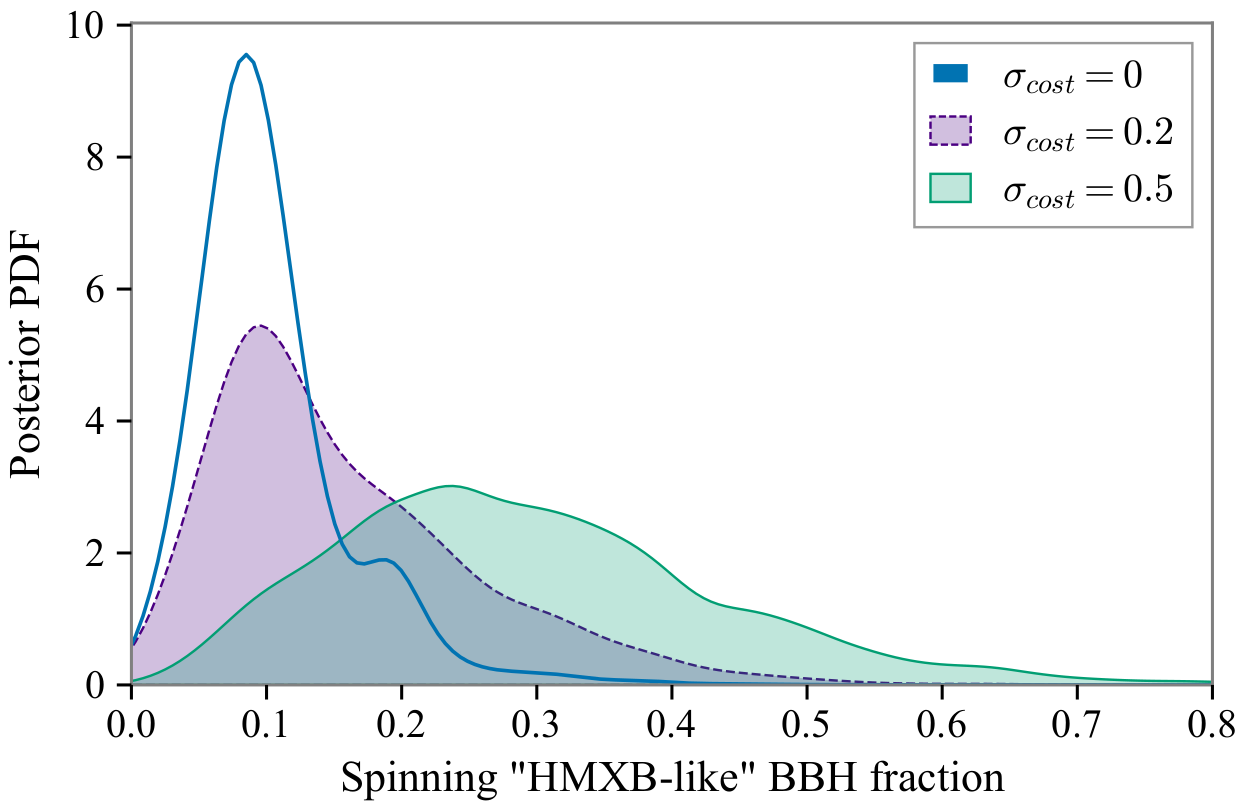
\includegraphics[width=\textwidth]{./images/tensionspinHMXBHlike.png}	
	\end{minipage}
	\caption{\emph{Left:} cumulative distribution function (CDF) of primary and secondary black hole spins detected with the gravitational wave detectors in GWTC-2 (orange) compared with the ones of the LMXBs (pink) and HMXBs (blue). In black the prior beta distribution used for the fits. The spin distribution of the black hole binaries is in tension with the ones inferred from the X-ray binaries. \emph{Right:} Posterior distributions of the fraction of black hole binaries that could have evolved from a HMXB-like configuration. The more the primary spin is aligned to the orbital angular momentum (smaller $\sigma_{\rm \cos \theta}$ values, see Sec.\ \ref{subsec:tensionspin} for more infos) and the more the HMXB configuration is irrelevant in the underlying population \cite{HMXBH_spins2021}}\label{fig:tensionspin}
\end{figure}


\subsection{Strong tension in the spin distribution}\label{subsec:tensionspin}
The spin distribution of the black holes detected with the gravitational waves (including both primary and secondary black holes) seems to be in tension with the spin distribution of the black holes detected in the X-ray binaries, as clearly visible in the left panel of Fig.\ \ref{fig:tensionspin}. The black hole binaries appear to host slowly spinning black holes, whereas both the LMXBs and HMXBs contain fast rotating black holes. Beta distribution fits to the observed spins of the LMXBs (pink) and HMXBs (blue) denote that the two types of X-ray binaries have spin distributions consistent within 90 \%. A single beta distribution fitted to the LMXBs and HMXBs altogether exhibits a disagreement at the 99.9 \% level with the spin distribution of the black hole binaries observed with the gravitational waves (orange).\cite{HMXBH_spins2021}\\

The three HMXBs considered here (LMC X-1, M33 X-7 and Cyg X-1) host very fast spinning black holes $\chi \gtrsim 0.8$: if they produce a black hole binary in the isolated binary evolution scenario, it is likely that the mass transfer processes and tidally locking will align the spins to the orbital angular momentum of the binary \cite{Kalogera2000_spinaligned}. However, supernova kicks may still cause a tilt in the spin orientation, allowing to model the spin tilts angles $\theta$ with a half-Gaussian in $\cos \theta$, peaked at aligned spins $\cos \theta = 1$  with some standard deviation $\sigma_{\rm \cos \theta}$: the larger the tilt angle, the larger the standard deviation \cite{spintiltmodel_Talbot2017}. 

It is possible that a sub-population of the black hole binaries evolved through a HMXB-like configuration; Bayesian inference methods can be used to put upper limits to the fraction of black hole binaries belonging to it. One of the input parameters of the inference method is the effective spin $\chi_{eff}$ i.\ e.\ the mass-weighted component of the spins aligned to the orbital angular momentum (see Eq.\ \ref{eq:chieff}). Determining the upper limits in the sub-population weight means assuming that the $\chi_{eff}$ is mainly determined by the spin of the primary black hole. Therefore, a black hole binary coming from a HMXB-like configuration will be modeled with secondary spin narrowly peak around zero and primary spin distributed with the half-Gaussian in $\cos \theta$. 

The right panel in Fig.\ \ref{fig:tensionspin} shows the results of three possible estimates of the sub-population weight allowing for three different maximum tilts of the primary spin: no tilt ($\sigma_{\rm \cos \theta} = 0$), $\lesssim 12^{\circ}$ tilt ($\sigma_{\rm \cos \theta} = 0.2$) or $\lesssim 30^{\circ}$ tilt ($\sigma_{\rm \cos \theta} = 0.5$). The more the primary spin is forced to be aligned, the less the HMXB configuration is relevant in the formation history of the black hole binaries. The fraction of binaries belonging to the sub-population of HMXB-like binaries is only $< 19 \% $ for aligned spins, growing to $< 30 \%$ for slightly tilted spins ($\sigma_{\rm \cos \theta} = 0.2$) and up to $< 48 \%$ for mildly tilted spins ($\sigma_{\rm \cos \theta} = 0.5$).\\

The evolutionary mechanisms necessary to create a rapidly spinning primary in a system that forms a black hole binary merging within a Hubble time are still under investigations. One of the proposed channels involves a stable mass transfer event from a Main Sequence donor to a Main Sequence accretor. If the angular momentum transport is inefficient inside the star and the mass transfer can remove its envelope tidally-locking the system, a lot of the angular momentum can be maintained in the core of the donor star. After a similar mass transfer, the donor will rapidly become a Wolf-Rayet and eventually produce a fast spinning black hole \cite{spinfastBH_Qin2019}. Population synthesis studies coupled with detailed stellar evolution models showed that only $\lesssim 12 \%$ of the HMXB binaries formed in this way had the right combination of parameters to evolve into a black hole binary that merges via gravitational wave emission within a Hubble time. Overall, only $\lesssim 20 \%$ of the merging black hole binaries seem to undergo this kind of evolution, in agreement with the upper limit of $\lesssim 30 \%$ found for slightly tilted spins \cite{HMXBHspins2022}.





\chapter{Wolf-Rayet - black hole binaries}
\paragraph{An intermediate evolutionary stage}
The systems composed of two massive stars are the best possible progenitors for the black hole binaries observed with the gravitational wave detectors: the stars are massive enough to form a black hole ($\mzams \gtrsim 15-25~\msun$ at solar metallicity, according to the single stellar evolution \cite{Limongi2017_handbookSN}) and will likely undergo at least a mass transfer episode (82 O-type stars with mass $\sim 15-60~\msun$ observed in six Galactic open cluster revealed that $70 \%$ of the massive stars are born in binaries, close enough to allow mass transfer interaction \cite{Sana2012}). 

Population-synthesis studies suggest that at least one mass transfer episode is necessary to shrink the orbit and allow the coalescence within a Hubble time \cite{spera2019_mergingBBH}. On the one hand, it is difficult to predict the type of mass transfer and the fate of the binary because they strongly depend on the orbital separation and on the details of the stellar evolution, as shown in Fig.\ \ref{fig:Sana2012MTfate}. On the other hand, usually the mass transfer and the strong stellar winds strip the hydrogen envelope of the massive stars, producing a Wolf-Rayet star. If the right conditions are met, the  Wolf-Rayet can form with a black hole companion: the strong winds of the Wolf-Rayet can power the accretion disk of the black hole and make the system visible as a X-ray binary.

\paragraph{Chapter outline}
This chapter reviews the theory of the single stellar evolution and of the main mass transfer processes (wind-fed accretion, Roche lobe overflow and Common Envelope) to better understand the evolution of the Wolf-Rayet - black hole binaries. I will report the observed properties of the known Wolf-Rayet - black hole systems, discussing the difficulties in the parameter estimation. Finally, I will describe the Cyg X-3 system: the only known Galactic Wolf-Rayet - black hole binary.


\begin{figure}[h!]
	\centering
	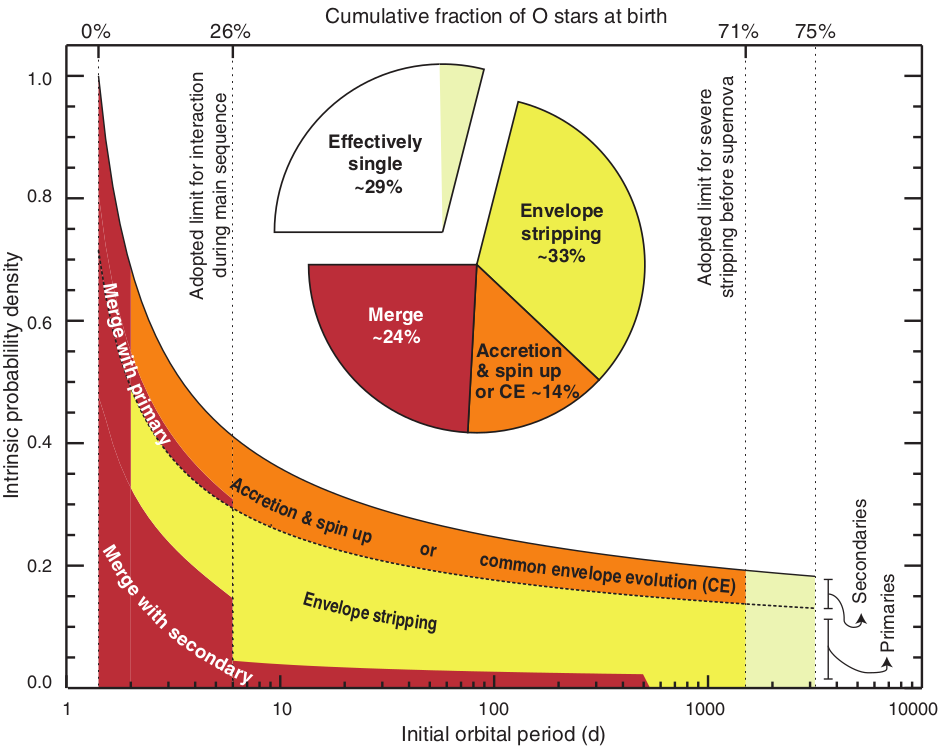
\includegraphics[width=.65\textwidth]{./images/Sana2012MTfate.png}
	\caption{70\% of O-type stars will be part of a binary with initial period < 1500 days and will undergo at least one mass transfer process. The type of mass transfer and the fate of the binary will depend on the details of the single stellar evolution and on the orbital separation. \cite{Sana2012}}\label{fig:Sana2012MTfate}
\end{figure}


%%%%%%%%%%%%%%%%%%%%%%%%%%%%%%%%%%%%%%%
%%%%% END OF "DEFINITIVE" PART %%%%%%%%
%%%%%%%%%%%%%%%%%%%%%%%%%%%%%%%%%%%%%%%

% paperino

%%%%%%%%%%%%%%%%%%%%%%%%%%%%%%%%%%%%%%%%%%%%%%%%%%%%%%%%%%%%%%%%%
%%%%%%%%%% WORK IN PROGRESS BELOW %%%%%%%%%%%%%%%%%%%%%%%%%%%%%%%
%%%%%%%%%%%%%%%%%%%%%%%%%%%%%%%%%%%%%%%%%%%%%%%%%%%%%%%%%%%%%%%%%



\section{Wolf - Rayet stars}
\subsection{Spectral classification}
WN, WC etc. 
Anche M-L relation?
Stellar winds empirical by Nugis and Lamers
\subsection{Single stellar evolution}
Little recap of single stellar evolution on what is and how evolves a WR, underlying e.g. the typical progenitor masses and the importance of the stellar winds.\\

SSE descritta nel dettaglio fino alla massa del CO e alla sua depletion ad alte metallicità, argomento che verrà ripreso nella spiegazione delle CCSNe in SEVN


PLOT: SSE of 30 and 40 Msun with Z=0.015 and 0.02 to show influence of mass and stellar winds.

\section{Mass transfer theory}
Short overview of the main binary processes, with particular attention to the wind accretion, Roche lobe overflow and common envelope


\section{Observed candidates of Wolf-Rayet - black hole systems}\label{sec:WRBHobserved}
The core is the paragraph I already wrote for the Computational Astrophysics exam (a table with the observed properties and short explanations on the uncertainties of the measurments). Brief review of the literature on possible evolutions of the systems as GW mergers.\\



%%%%%%%%%%%%%%%%%%%%%%%%%%
%%%%%%%%%%%%%%%%%%%%%%%%%
\begin{figure*}
	\begin{threeparttable}
		\begin{tabular}{llccccc}
			\toprule
			Host galaxy & Name & BH mass [$\msun$] & WR mass [$\msun$] & Period [h] & $t_\textup{GW}$ [Gyr]  &Z [$\zsun$] \\
			\midrule
			IC 10 & IC10 X-1 & 23-33\tnote{a} & 35\tnote{b} & 34.9\tnote{a} & 3.5  & 0.22 \\
			NGC 300 & NGC300 X-1 & 13-21\tnote{d} & 26\tnote{c} & 32.8\tnote{d} & 2.9  & 0.19 \\
			M101 & M101 ULX-1 & 20-30 & 19& 196.8 & 348 & 0.17 \\
			Milky Way & Cyg X-3 & 3 & 7 &4.8 & 0.017 & 0.31 \\
			NGC 4490 & CXOU J123030.3+413853 & - & - & 6.4 & 0.038  & 0.23 \\
			NGC 253 & CXOU J004732.0-251722.1 & - & - & 14.5 & 0.33  & 0.24 \\
			Circinus & CG X-1 & - & - & 7.2 & 0.051  & 0.10 \\	
			\bottomrule 	
		\end{tabular}
		\begin{tablenotes}[para]
			\item[a]\cite{IC10X-1_Silverman2008} 
			\item[b]\cite{IC10X-1_Clark2004_WRmass}
			\item[c]\cite{NGC300X-1_Crowther2010} 
			\item[d]\cite{NGC300X-1_Binder2021_BHpreciso}
		\end{tablenotes}
		\centering
		\captionof{table}{Properties of the seven WR-BH candidates. The table is inspired by \cite{observations}. $t_\textup{GW}$ is an order-of-magnitude estimate calculated assuming $M_{1,\rm BH} = M_{2,\rm BH} = 10~\msun$, given the uncertainties in the mass determination discussed in Section . The other parameters are extracted from the above referenced papers and from \cite{M101ULX-1_Liu2013} (M101 ULX-1), \cite{Cyg-X3_Zd2013} (Cyg X-3), \cite{NGC4490cand_Esposito2013c} (CXOU J123030.3+413853), \cite{NGC253cand_Maccarone2014} (CXOU J004732.0-251722.1), \cite{observations} (CG-X1), \cite{observationsZSFR_Mapelli2010a} (Z).} \label{tab:observations}
	\end{threeparttable}
\end{figure*}
%%%%%%%%%%%%%%%%%%%%%%%%%
%%%%%%%%%%%%%%%%%%%%%%%%%

\section{Cyg X-3}
Review of Koljonen+2017 and discussion on why values of Zdiarski+2013 are not reliable and we don't use them. Also describe it is in the MW and how we determined its metallicity and distance.
\subsection{Properties}

\subsubsection{Observations and identifications}
Cyg X-3 lies in the galactic plane therefore no optical/UV counterpart has been detected yet due to interstellar absorption (\cite{CygX-3_Koljonen2017}). Thus we know that the companion is a WR only by observing its IR spectrum. Using IR and X-ray emission lines, the companion is a low-mass BH or a NS.

\subsubsection{DIstance and metallicity}
\textbf{McCollough2016} on the galactic plane ($l=79.84^\circ, b=+0.70^\circ$). Distance 7.4 $\pm$ 1.1 kpc or, but less, probable, 10.2 $\pm$ 1.2 kpc. Distance estimated by looking at the "little friend" of Cyg X-3 i.e. a nearby Bok globule that was observed in X-ray by Chandra and then followed up with Submillimetric observations. This Bok globule is a 2-24 \msun gas+dust cloud confined in a 0.2 pc that scatters towards us the X-ray radiation produced in the nearby X-ray binary. Assuming that the velocity shift of the CO line is due only to the galactic rotation, the authors could use a tool for modeling the motion on the galactic disk and reconstructed a distance of 7.4 or 10.2 kpc (two values because of possible errors in the tool evaluation but the first is more probable).\\

We expect that Cyg X-3 was born in the star-forming region associated to the Bok globule and then the SN kick that formed the BH expelled the system from the Bok globule. Given that the binary is $\sim 1$ kpc away from the Bok globule and the lifetime of the WR, therefore the time elapsed from the SN, is $\sim 1-5 \times 10^6$ years, the authors estimate a SN kick of $\sim 190-980$ km/s, in agreement with some upper and lower independent constraints.\\

To model its metallicity we use the metallicty gradient of the MW that was obtained by \textbf{Lemasle2018} using Gaia data of metallicity and distance of 25 Cepheids. They found \[[Fe/H]=-0.0447*d_{\rm Galacto}(kpc) + 0.3522\]. By tringulation, the galactocentric distance of Cyg X-3 is $d_{\rm Galacto} = 9.85$ kpc ($l=79.84^\circ$, heliocentric distance = 7.94 kpc from Lemasle 2018 and relative distance of Cyg X-3 = 7.4 kpc from the measurements on the BOk globule carried out by McCollough 2016). We therefore obtain \[[Fe/H] = -0.088095\] and, assuming that the metallicity distribution of the Sun is universal, we can convert such value to the metal mass fraction using \[[Fe/H] = log(Z/X)_* - log(Z/X)_\odot\] i.e. we obtain \[Z_* = 0.91567 \zsun\]. If we assume \zsun=0.02 we get $Z_*=0.0183$ but if we assume \zsun=0.01524 we get $Z_*=0.01395$.

\subsection{Period}
\subsubsection{Singh 2002} 4.8 hours. We take a larger range i.e. 4.5 - 5.1 hours, that combined with the possible mass ranges for WR and BH results in a semimajor of $a \sim 3-4 $ Rsun


\subsection{Mass ranges}
\subsubsection{Koljonen \& Maccarone 2017} I used WR = 8 - 14 \msun, BH = 3. - 10 \msun \\

They derived: ?? \\

Model: X-ray emission from compact object ionizes the stellar wind of the WR and causes the emission lines visible in the NIR (1-2.4 $\mu$m). They use a non-LTE model for the atmosphere of the WR to reproduce the continuum + emission lines in the NIR. \\

Semimajor axis according to my model: Minimum possible a=3.052 Rsun with P=4.5 hours and Mtot = 8+3=11 \msun .  Maximum possible a=4.303 Rsun with P=5.1 hours and Mtot = 14+10=24 \msun 


\subsubsection{Zdziarski 2013} \cite{Cyg-X3_Zd2013} I used WR = 7.5 - 14.2 \msun, BH = 3 - 4.5 \msun \\

THey derived:WR = 7.5 - 14.2 \msun, Compact object = 1.3 - 4.5 \msun and then Belczynski 2012 assumed as MminBH = 2 \msun\\
\\

\subsubsection{Procedure}
Vogliono risolvere un sistema a due variabili \mdot e MWR dove le due equazioni sono eq. 3 e eq 6 nel paper, che, combinate con altri dati osservativi e combinazioni, diventano le equazioni 7 e 8.

La prima descrive il rallentamento della binaria a causa del momento angolare trasportato via dal vento che lascia il sistema. Tale equazione lega Mdot, MWR+MCO, Pdot/P e di essa conosciamo $Pdot/P = 1.03+- 0.02 x 10^{-6} ~ \rm yr^{-1}$ da Kitamoto (comunicazione privata) e possiamo legare MCO alla massa della WR attraverso il mass ratio della binaria q che altro non è che il rapporto tra i due picchi delle due curve di rotazione

\[q = Mcompact/MWR = KWR / Kcompact \sim 0.23\] 

Problema: Ko17 evidenziano che Zd13 hanno usato i dati di Hanson2000 che aveva usato come tracciante per il moto orbitale la linea di assorbimento HeI 2p-2s e che purtroppo è molto probabile che questa linea NON sia un tracciante per il moto orbitale bensì per il campo di velocità del vento della WR. Inoltre, lo spettro usato era stato preso nel 1999 durante un outburst, quando era presente anche una doppia linea di emissione He I 2p-2s a compilcare il tutto. 




Semimajor axis according to my model: Minimum possible a=3.005 Rsun with P=4.5 hours and Mtot = 7.5+3=10.5 \msun .  Maximum possible a=3.96 Rsun with P=5.1 hours and Mtot = 14.2+4.5=18.7 \msun 


\chapter{Models and simulations with SEVN2}
\section{The SEVN2 population-synthesis code}
Interpolates PARSEC tables, describe winds, criteria for identifying a WR, explain how, explain details of mass transfer, explain assumption on the pessimistic case, explain the three kick models, 
\subsection{CCSN}
explain the three CCSN models (use histograms)\\
PLOT: histogram with compact remnants with different SN models\\
(PLOT: histogram with compact remnants with different kick models )

\section{Initial conditions for simulations}
Describe the distributions of masses, periods, eccentricities from which I derived the 1 million simulations. Scheme with the parameter space explored

\chapter{Results}\label{sec:results}
\section{> 90 \% GW-BBH undergo WR-BH configuration}
4 tabelle per i 4 modelli di kick che mostrano che nonostante si varino CCSN e metallicità è incontrovertibile che la WR-BH sia una configurazione obbligata.

\section{Fiducial model}
In dettaglio mostrare hist2d di a vs m1+m2 per progenitori, inizio WR-BH, remnants, m1+m2 vs tgw, m1 vs m2 progenitor, m1 vs m2 remnant.\\
In dettaglio analizzare evoluzione di Cyg X-3 con i trasferimenti di massa e le proprietà di osservabilità tipo il RL filling e la divisione in due/tre famiglie. Grafici: M1 VS M2, RL1fill vs RL2fill, RL1fill vs M1 per discutere il wind-fed, grafico periodo vs tempo in WR-BH per discutere tempo osservabilità, evoluzione di una singola binaria rappresentativa per tipo di mass transfer (RLO+RLO+CE, RLO +CE e CE+CE)

\section{Role of metallicity}
Comparare con stesso kick unified + 265 + CCSN = compact ma scegliendo Z=0.02 e discutere il diverso tempo evolutivo, canali e durata mass transfer e proprietà.
Mostrare gli hist2d per a vs m1+m2 per progenitor e remnant e mostrare che sono gli stessi.\\
Poi usare come prima tre binarie rappresentative per i 3 tipi di mass transfer di Cyg X-3 e discutere le differenze rispeto a Z=0.15. Mostrare anche le differenze nei grafici M1 VS M2, RL1fill vs RL2fill.


\section{Role of the kicks}
Mostrare per Z=0.015 + CCSN= compact che diversi kicks cambiano principalmente il semiasse finale, scatterando molto di più i risultati delle GW-BBH ma lasciando quasi inalterati i candidati Cyg X-3 e la loro evoluzione. Mostrare i 4+4 grafici di a vs m1+m2 remnant e di m1vsm2 di Cyg X-3.

\section{Role of CCSN model}
Comparare prima con il kick fiducial unified+265 e Z=0.015 i tre modelli di CCSN e mostrare per ciascuno 2 grafici: M1 VS M2 per Cyg X-3 e a vs m1+m2 dei remnants. Ricordando le differeze iniziali nei modelli, spiegare le differenze.


\section{Probing the parameter space}
Mostrare a vs m1+m2 remnant e m1vsm2 Cyg X-3 a set di 3 CCSN variando i tre kick prima con Z=0.015 e poi con Z=0.02. Discutere come l'evoluzione di Cyg X-3 rimanga molto simile ma hobbs pure + rapid/delayed scatteri moltissimo le proprietà dei remnant





\section{Compare with Belczynski+2013}
??? Ha senso??




\chapter{Conclusion}
\begin{itemize}
	\item WR-BH as mandatory intermediate configuration needed to form GW-BBH at solar metallicity. Implication for spins (?)
	\item Well-defined properties for Cyg X-3 systems (say which), less defined for GW-BBH but quite well-constrained.
	\item At least a CE is needed + another CE or a stable RLO. Optional a third stable RLO for Cyg X-3 like systems. To be investigated if it is true also for GW-BBH but we think this may be representative for GW-BBH in the region of Cyg X-3
	\item CCSN introduces the most uncertainties in the masses of the remnants, thus selecting the evolutionary paths (e.g. the delayed almost completely removes the stable mass transfer channels)
	\item The kicks most favour the semimajor and when combined with rapid/delayed spread a lot the results
	\item Metallicity changes the stellar evolution and also spreads the results, even though a little less. Most importantly, it may transform the second mass transfer from RLO stable + CE into one single CE after a long RLO, all because the donor MS is able to expand/contract differently therefore R>RL long enough to become unstable before re-entering the RLO
\end{itemize}






\chapter{Annotazioni/Bozza}
With the fiducial model i.e. Z=0.015, SN=compactness, kick=unified, sigma = 265
\begin{itemize}
	\item Probability to form a WR/BH(cyg x-3 like) system in principle out of all binaries
	\item Probability to form a GW-BBH WR/BH(cyg x-3 like) system in principle out of all binaries
	\item Probability a WR-BH(cyg x-3 like) system has 2RLO/RLO+CE/2CE
	\item Probability it is visible in the WR-BH(cyg x-3 like) configuration?
	\item Time from system born, time from WRBH born, time to BHBH, time to merge all as a function of observed period and total mass
	\item probability it is observed as RL filling/wind fed system as function of semimajor
	\item evolutionary pathaway of WRBH (cyg x-3)
\end{itemize}


\subsection{Parameter space to explore}
OPtimistic o pessimistic scenario for RLO \\
Z= 0.02 and Z=0.015\\
SN = rapid, delayed, compact \\
Kicks = hobbs pure + sigma = 70 (Atri 2019, from median of 107 km/s) \\
Kicks = hobbs pure + sigma = 265 \\
+ fiducial \\
+ Belczynski


\subsection{Compare with Belczynski}
Evolve with Z=0.02, SN=rapid, kick=sigma 265 + fallback as Fryer.


Belczynski considered Z=0.02 and sigma=265 always and always obtained a BBH. He varied different parameters though:
\begin{itemize}
	\item rapid + hobbs + fallback = 14.2 WR + 4.5 BH --> 7.4 BH + 4.5 BH
	\item rapid + hobbs + fallback = 14.2 WR + 4.5 BH --> 8 BH + 4.5 BH (\textbf{NugisLamers2000 winds})
	\item rapid + hobbs pure = 14.2 WR + 4.5 BH --> 7.4 BH + 4.5 BH
	\item delayed + hobbs + fallback = 14.2 WR + 4.5 BH --> 3.9 BH + 4.5 BH
\end{itemize}

Cioè con il rapid model, a prescindere dal kick model (=con o senza fallback) ottiene sempre che una WR di 14.2 iniziali diventa un BH di 7.4-8 Msun. Invece con il delayed (e il fallback) il BH è molto più leggero.\\

In ogni caso predicono che il sistema starà in configurazione WR-BH per 0.64 Myr

\subsection{Notes on how SEVN works/how to interpret things/where to focus}
Taglio della tesi: 
\begin{itemize}
	\item Primo aspetto/paper: per diventare GW-BBH a metallicità locale è NECESSARIO passare per la fase di WR-BH. Ammesso e non concesso (forte assunzione) che i GW-BBH osservati attualmente provengano da isolated channel a questa metallicità, ciò significa che gli spin devono essere gli stessi e questo sarebbe un grosso problema, visto che attualmente Vicky \& Kalogera in apple e oranges hanno sottolineato che non è assolutamente la stessa cosa...
	\item Secondo aspetto/paper: cyg x-3 evolve così o colà a seconda del parameter space ma sembra avere proprietà iniziali/finali molto ben definite negli hist2D e ciò rende i risultati abbastanza well-constrained
	\item Per rendere questo risultato un po' più solido bisognerebbe anche esplorare le BH-NS, tutte le WR-BH che non sono cyg x-3, a metallicità più basse
\end{itemize}

Cosa non è chiaro/è da testare

 
\begin{itemize}
	\item Kick = Unified + sigma = 70 km/s non ha senso perché unified è stato calibrato per riprodurre le osservazioni a partire dalla maxwelliana di hobbs. Pertanto è stato pensato per estrarre il kick da una maxwelliana di 265 km/s e poi diminuirne la magnitudine in base a ejecta e massa del remnant. Se parto già con una sigma di 70 sto già estraendo dei kick bassi, non posso diminuirli ancora di più...
	\item Il fatto che con hobbs puro io abbia un sacco di merging BBH ad alti semiassi posso provare a spiegarlo guardando all'eccentricità delle binarie, magari c'entra quanto vicine al periastro passano oppure no
	\item Overcontact binaries da testare perché passano quasi tutte per di là.Inoltre Giuliano spiega: questione overcontact binary: conosco bene questi casi e sono proprio alla base dell’ultima “importante” modifica di SEVN. 
	Precedentemente questi casi andavano tutti a finire in merger o CE, ma ci siamo resi conto che in BSE/MOBSE questo check è disabilitato mentre c’è un RLO. Ora è cosi anche in SEVN. 
	Ho già controllato che questi casi soprattutto durante un HG sono presenti anche in BSE/MOBSE. 
	
	Quindi in sostanza ogni volta che il Raggio>RL e quindi c’è un RLO consideriamo per la stella  un raggio effettivo pari a quello del RL per tutti i vari processi (venti,tides) mentre il Raggio della stella è usato 
	solo per stimare il rate di mass transfer usando l’equazione 58 in Hurley02.
	
	Se questo sia il modo migliore per gestire il mass transfer non saprei, probabilmente no, ma si inserisce nel discorso piu ampio di andare oltre le prescriptions di Hurley. 
	Abbiamo gia visto che lasciare che questi oggetti mergono in realtà è un assunzione che non funziona soprattuto considerando i merge rate delle neutron stars. 
	
	Per fare un discorso pratico e concreto quello che ottieni in SEVN è consistente con Hurley e BSE/MOBSE ed è solo una conseguenza del modello di RLO adottato. 
	Alla fine non ha nemmeno troppo senso avere plot in cui mostri il raggio durante il RLO perché per SEVN in questi casi il raggio effettivo della stella è pari a RL. 
	\item la SN compact è descritta come nel paper della mapelli https://arxiv.org/pdf/2005.03055.pdf dove il grafico in basso è stato fittato con due distribuzioni. Se nel file .sh il parametro -1 è settato, allora la treshold zeta2.5 non è 0.3 come nel paper della mapelli ma viene estrapolata randomicamente da quelle distribuzioni (o una roba del genere). La SN= compactness è MOLTO biasata nel creare BH invece che NS
	\item per la SSE delle pure He posso confrontare la stessa stella se tipo mi faccio printare anche la colonna "zams" che mi dice qual è la traccia che sta usando per l'interpolazione (a seconda della tabella usata)
	\item Capire nel dettaglio le differenze tra Z=0.02 e Z=0.015
	\item Focus sul final fate dopo la WR-BH per un confronto con Belczynski
	\item controllare le incertezze sulle masse di KO17!!! Specialmente la metallicità usata per la M WR dalla relazione M-L
	\item Pessimistic/optimistic case riguarda la possibilità che una stella in HG possa entrare ed eventualmente sopravvivere ad un CE (optimistic) oppure si fonda direttamente con la compagna nell'ipotesi di assenza di un core ben definito (pessimistic)
\end{itemize}

They predict:\\
\begin{itemize}
	\item WR progenitor of 50 Msun produces WR of 14.2 Msun with R=1.2 Rsun and Rlobe = 1.8 in a=3.8 Rsun orbit with a BH of 4.5 Msn as companion
	\item mass loss rates for the WR taken from Hurley 2000 + Hamann \& Koesterke 1998 (theoretical)
	\[\dot{M} = 10^{-13}(L/L_\odot)^{1.5} \msun \yr^{-1}\]
	\item WR lives for 0.64 Myr and becomes a 8.2 Msun WR with CO core of 6.2 Msun and orbit expanded to a=5.6 Rsun. 
	\item rapid core collapse for the WR leads to fallback=1 but with the 10\% of the gravitational mass lost due to neutrinos we obtain a secondary BH of 7.4 Msun with NO NATAL KICK (because the fallback is maximum therefore it is fully damped), slightly wider orbit of a=6 Rsun and e=0.07.
	\item the final BHBH of 7.4 Msun + 4.5 Msun has a chirp mass of 5.0 Msun and will merge in 500 Myr.
\end{itemize}

\textbf{Different wind}:\\
\begin{itemize}
	\item Use wind taken from Nugis \& Lamers 2000 as done in Zdziarski i.e. by selecting the ones for WR stars with the desired masses (empirical based on 64 WR in the MW. In particular in the mass range I am interested, out of the 34 observed WR, 19 were mostly in a binary system)
	\[\dot{M} = 1.9\times10^{-5}(M_{WR}/14.7\msun)^{2.93} \msun \yr^{-1}\]
	\item Slight increase in the BH formed after the WR (8 Msun instead of the previous 7.4 Msun. Probably because they are lower than the theoretical ones so they retain more mass i.e. they form a heavier BH in the end). 
	\item No other appreciable changes
\end{itemize}

\textbf{Different kick}:
\begin{itemize}
	\item if no fallback the probabilty to form a merging BHBH system reduces from 100\% sure to only 68\% because some systems are disrupted by the larger kicks
\end{itemize}


\textbf{Different SN}:
\begin{itemize}
	\item delayed model forms a lighter BH (3.9 Msun instead of the 7.4 Msun) because the delayed explosion allows more mass to escape and not to accrete back. This also lowers the formation efficiency to 50\% 
\end{itemize}



\section{Compactness model implemented in SEVN}
As explained in Mapelli+2020 \cite{mapelli2020_compactness}, the compactness model in SEVN uses the final CO mass to interpolate the compatness parameter

\begin{equation}
	\xi_{2.5} = 0.55 -1.1 \left(\frac{1 \msun}{m_{\rm CO}}\right)
\end{equation}

where the above formula is derived with fits to FRANEC data.\\

Patton and Sukhbold 2020 \cite{COcollapse}, in the bottom figure of Fig. 3, provide the probability that a star with a given compactness parameter undergoes an explosion or implosion. We fitted to that data a probability distribution and use it to randomly decide whether out star with that compactness will explode, forming a NS, or will implode, forming a BH.\\

After the compact remnant is formed, 



\section{Pipeline}
\begin{itemize}
	\item Su demoblack result.py, read.py e WRBH.py per generare i file WRBH, BHBH, BHNS, result.txt e le cartelle dataframes e copied. Il tutto viene salvato in una cartella che identifica la simulazione e si chiama tipo 1mln\_Z015\_com\_unified265
	\item Quest'analisi include nei file WRBH, BHBH e BHNS tutti i corrispondenti candidati usando come criterio di classificazione unicamente la PhaseBSE e NON la massa
	\item La cartella tipo 1mln\_Z015\_com\_unified265 viene copiata sul pc
	\item Si fa debugging per estrarre correttamente i BH, cioè scegliendo se considerare come "veri" BH anche i BH con massa < 3 che si originano dalla PPISN. Per fare ciò si fanno andare gli script result2.py, read2.py e WRBH2.py scegliendo, a seconda, l'opzione desiderata per il debugging: debug= 'ppisn' sceglie come massa minima per i BH in Cyg X-3 quella pari a ?? in base a ?? mentre l'opzione debug='real' seleziona come BHBH e BHNS solo i sistemi dove il BH sia un oggetto compatto con massa > 3
\end{itemize}





\section{Results Cyg X-3}
Present results with different parameters (SN model and metallicity) and show how they impact on the evolution in general. Underline the main evolutionary paths (RLO/CE) and progenitors and remnant properties (like the computational exam)

Then show detailed evolution for Cyg X-3 only, showing differences with Belczynski 2013.





\printbibliography[heading=bibintoc]
\end{document}


